% !TEX root = ../notes_template.tex

\chapter{코시 적분 정리와 응용}

복소미분은 어느정도 익숙해졌으니 이제 적분으로 관심을 돌려보자.
이 장에서는 복소해석학에서 매우 중요한 다음 정리를 배울 예정이다.
\begin{center}
\fbox{
코시 적분 정리
}
\end{center}
``경로적분''을 정의하는 것으로 시작하여 나중에 코시 적분 정리를 증명할 예정이다.
왜 경로적분과 코시 적분 정리가 왜 그렇게 중요한지 의문을 가질 수 있다.
복소평면에서 적분의 중요성은 복소해석함수의 더 큰 이해로 이어지기 때문이다.
예를 들면, 복소해석함수는 무한번 미분가능하다는 본질적인 성질이 있다.
이 장에서 다음 주제들을 중심으로 공부해보기로 하자.
\begin{enumerate}
\item[(1)] 경로적분의 정의와 성질
\item[(2)] 경로적분의 기본정리
\item[(3)] 코시 적분 정리
\item[(4)] 코시 적분 정리의 응용
\begin{enumerate}
\item 부정적분의 존재성
\item 복소해석함수의 무한번 미분가능성
\item 리우비우 정리와 대수학의 기본정리
\item 모레라 정리
\end{enumerate}
\end{enumerate}

\section{경로적분의 정의}

일반적인 미적분에서 연속함수 $f: [a,b] \to \mathbb R$가 주어질 때
\begin{equation}\label{eq-3-1}
\int_a^b f(x)dx
\end{equation}
의 의미는 명확하다. 이제 이를  일반화하여 복소수까지 확장하고
주어진 복소수 $z$, $w$에 대하여
\[
\int_z^w f(\zeta)d\zeta
\]
에 의미를 부여하길 원한다고 하자.
$z$에서 $w$까지를 어떻게 해석해야 할까?

$\mathbb R$에서 $a<b$이면, 실수 $a$부터  실수 $b$까지
가는 경로는 한가지 뿐이다.  
따라서 실수의 경우는 단지
\begin{itemize}
\item[(1)] $a<b$이고,
\item[(2)] 연속함수 $f:[a,b] \to \mathbb R$
\end{itemize}
의 경우만 생각하면 충분하다.

하지만, $z$와 $w$가 복소평면 위의 점이면
그림 \ref{fig-3-1}과 같이 많은 경로에 대하여 적분을 생각할 수 있다.

\begin{figure}[!h]
\begin{center}
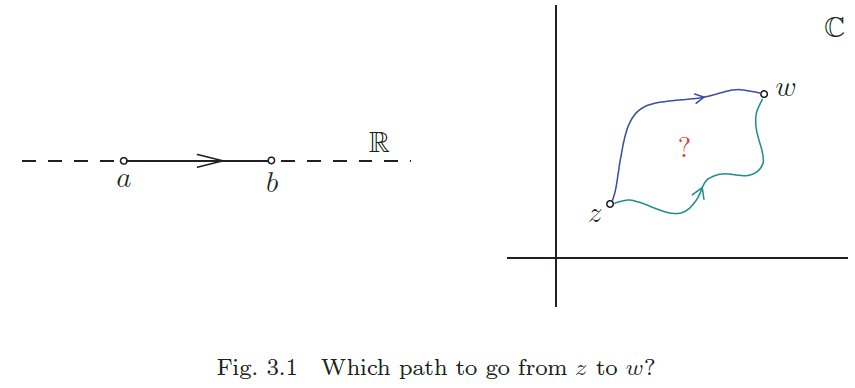
\includegraphics[width=0.8\textwidth]{./SaltChapter/fig-3-1}
\end{center}
\caption{$z$에서 $w$까지 어떤 경로로 가야할까?}
\label{fig-3-1}
\end{figure}

그러므로 복소수의 경우는 끝점 $z$와 $w$ 외에
$z$에서 $w$까지의 경로 $\gamma$도 지정하고,
실수의 경우를 나타낸 식 \eqref{eq-3-1}를
다음과 같이 복소수에 대한 표현으로 바꾸도록 한다.
\[
\int_\gamma f(z)dz.
\]

이 표현을 ``경로''적분이라 부르며
계산을 위해 다음을 결정할 필요가 있다.
\begin{itemize}
\item[(1)] 정의역  $D(\subset \mathbb C)$와 $z, w\in D$
\item[(2)] 연속함수 $f:D\to \mathbb C$
\item[(3)] $z$와 $w$를 잇는 {\bf 매끄러운} 경로 $\gamma: [a,b] \to D$
\end{itemize}

$z$와 $w$를 단순히 연결하는 경로가 아니라  {\bf 매끄러운} 경로가
필요하다는 사실에 주목하자.
여기서 ``매끄럽다''는 의미는 무엇일까?
경로 $\gamma : [a,b] \to D$는 연속함수임을 상기하자.
$\gamma$는 실수부와 허수부 $x,y: [a,b] \to \mathbb R$로 나누어  쓸 수 있다.
\[
\gamma(t) = x(t) + iy(t), \quad t\in [a,b].
\]
$x, y$가 연속미분가능하면
경로 $\gamma$가 {\bf 매끄럽다}고 한다.
예를 살펴보자.

\begin{salt_example} \label{example-3-1}
$\gamma : [0,1] \to \mathbb C$를 
$\gamma(t) = t(1+i)$ ($t\in[0,1]$)로 정의하자.
그러면 $\gamma$의 실수부와 허수부  $x,y: [a,b] \to \mathbb R$는
$x(t)=t$, $y(t)=t$, $t\in [0,1]$이 된다.
$x, y$가 $[0,1]$에서 연속미분가능이므로 $\gamma$는 매끄러운 곡선이다.
그림 \ref{fig-3-2}를 참고하라.
\begin{figure}[!h]
\begin{center}
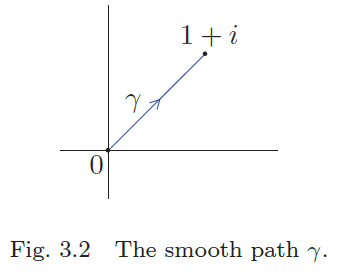
\includegraphics[width=0.4\textwidth]{./SaltChapter/fig-3-2}
\end{center}
\caption{매끄러운 곡선 $\gamma$}
\label{fig-3-2}
\end{figure}
비슷한 방법으로 다음과 같이 주어진 두 경로  $\gamma_1, \gamma_2: [0,2\pi] \to \mathbb R$를
생각하자.
\[
\gamma_1(t) = \exp(it), \quad \gamma_2(t) = \exp(2it), \quad t\in [0,2\pi].
\]
그러면 이 경로들의 실수부와 허수부는
$\cos t$, $\sin t$, $\cos(2t)$, $\sin(2t)$이고
모두 연속미분가능하다.
따라서 $\gamma_1, \gamma_2$는 모두 매끄러운 경로이다.
그림 \ref{fig-3-3}을 보자.
\begin{figure}[!h]
\begin{center}
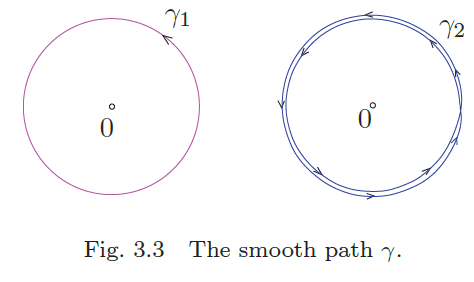
\includegraphics[width=0.6\textwidth]{./SaltChapter/fig-3-3}
\end{center}
\caption{매끄러운 곡선 $\gamma_1$과 $\gamma_2$}
\label{fig-3-3}
\end{figure}
두 곡선의 이미지 ($\gamma_1$과 $\gamma_2$의 치역)은 동일하다.
즉, 중심이 원점인 단위원이다.
\[
\{\gamma_1(t) \,:\, t\in[0,2\pi]\}  
= \{\gamma_2(t) \,:\, t\in[0,2\pi]\}  
= \{z\in\mathbb C \,:\, |z|=1 \}. 
\] 
그렇지만 $\gamma_1$과 $\gamma_2$는 다른 경로이다.
왜냐하면 함수로서 같지 않기 때문이다. 예를 들면
$\gamma_1(\pi) = -1 \ne 1 = \gamma_2(\pi)$.
\hfill $\diamondsuit$
\end{salt_example}

\begin{salt_remark} \label{remark-3-1}
경로 $\gamma: [a,b]\to \mathbb C$의 치역
\[
\{\gamma(t) \,:\, t\in[a,b] \}
\]
을 경로(또는 곡선) 자체라고 하는 것이 매우 일반적이며 편리하다. 
이 방식에서는 경로는 
복소평명에서의 원, 선분 구체적인 기하학적 개체가 되어 (함수라고 생각하는 것과 반대로),
쉽게 그려볼 수 있다.
이 방식에서는 {\bf 다른} 경로를 동일한 이미지로 볼 수 있어
모호함이 생긴다는 어려움이 있다.
\end{salt_remark}

경로적분의 정확한 정의는 다음과 같다.

\begin{salt_definition} \label{def-3-1}
다음이 주어질 때,
\begin{itemize}
\item[(1)] 정의역 $D$,
\item[(2)] 연속함수  $f:D\to\mathbb C$ (실수부와 허수부는 
$u,v: D\to\mathbb R$),
\item[(3)] 매끄러운 경로 $\gamma : [a,b]\to D$
(실수부와 허수부는 $x,y: [a,b] \to \mathbb R$),
\end{itemize}
경로적분을 다음과 같이 정의한다.
\begin{align} \label{eq-3-2}
\int_\gamma f(z)dz
&:= \int_a^b f(\gamma(t))\gamma'(t)dt \\
&:= \int_a^b \left( u(\gamma(t)) + iv(\gamma(t)) \right) \cdot
(x'(t) + iy'(t))dt \nonumber \\
&:= \int_a^b \left( u(\gamma(t)\cdot x'(t) - v(\gamma(t))\cdot y'(t) \right) \nonumber \\
&\quad +i \int_a^b \left(v(\gamma(t)\cdot x'(t) + u(\gamma(t))\cdot y'(t) \right) dt \nonumber.
\end{align}
여기서 마지막 두 적분은 우리에게 익숙한 실변수 연속함수의 리만적분이다.
\end{salt_definition}

다음과 같이 경로적분을 기하학적으로 해석할 수 있다.
\[
\gamma'(t) dt = x'(t)dt + iy'(t)dt
\]
이 항을 경로를 따라 국소적으로 변하는 증분으로 보자.
이 증분에 값 $f(\gamma(t))$ (국소적으로는 거의 상수이다)을 곱하고,
경로를 따라 더해나가면 결론적으로 적분값
\[
\int_a^b f(\gamma(t))\gamma'(t)dt
\]
에 도달하게 된다. 그림 \ref{fig-3-4}를 참고하라.

\begin{figure}[!h]
\begin{center}
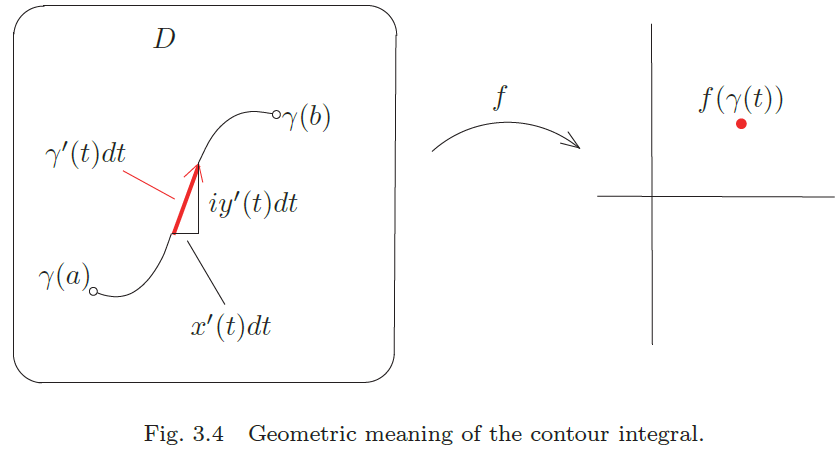
\includegraphics[width=0.8\textwidth]{./SaltChapter/fig-3-4}
\end{center}
\caption{경로적분의 기하학적 의미}
\label{fig-3-4}
\end{figure}

\begin{salt_example} \label{example-3-2}
다음과 같이 주어진 조건에 대하여
\begin{itemize}
\item[(1)] $D=\mathbb C$,
\item[(2)] $\gamma$는 $\gamma(t)= t(1+i)$ ($t\in[0,1]$)로 정의된 매끄러운 경로,
\item[(3)] $f = (z\to \bar z)$,
\end{itemize}
\begin{align*}
\int_\gamma f(z)dz &= \int_0^1 \overline{t(1+i)}\cdot (1+i)dt \\
&= \int_0^1 t(1-i)\cdot(1+i)dt
= \int_0^1 t(1^2-i^2)dt = \int_0^1 t(1+1)dt \\
&= 2\int_0^1 t\,dt = 2\cdot \frac{t^2}2 \Big|_0^1 = 2\cdot \dfrac12 = 1.
\end{align*}
\end{salt_example}

\begin{salt_exercise} \label{ex-3-1}
세 경로 $\gamma_1, \gamma_2, \gamma_3: [0,2\pi] \to \mathbb C$가 
$t\in[0,2\pi]$에 대하여 다음과 같이 정의된다고 하자.
\begin{align*}
\gamma_1(t) &= \exp(it), \\
\gamma_2(t) &= \exp(2it), \\
\gamma_3(t) &= \exp(-it).
\end{align*}
경로의 이미지는 모두 같지만, 다음 세 경로적분은 모두 다른 값을 가짐을 보여라.
\[
\int_{\gamma_1} \dfrac1zdz, \quad
\int_{\gamma_2} \dfrac1zdz, \quad
\int_{\gamma_3} \dfrac1zdz.
\]
\end{salt_exercise}

\begin{salt_exercise} \label{ex-3-2}
$f$가 영역 $D$에서 복소해석함수이고, $\gamma:[0,1]\to D$가 매끄러운 경로라 하자.
모든 $t\in[0,1]$에 대하여 다음을 증명하라.
\[
\dfrac{d}{dt} f(\gamma(t)) = f'(\gamma(t))\cdot \gamma'(t). 
\]
\end{salt_exercise}

우리는 종종 일반적인 구간 $[a,b]$를 사용하지 않고
매끄러운 경로가 $[0,1]$에서 매개변수로 정의된 것으로 가정하기도 한다.
왜 이런 가정을 해도 되는지 이유를 설명해보자.

$\gamma:[a,b] \to \mathbb C$와  $\tilde\gamma:[a,b] \to \mathbb C$가
매끄러운 경로라고 하자.
연속미분가능한 함수 $\varphi:[c,d] \to [a,b]$가
$a=\varphi(c)$, $b=\varphi(d)$이고 모든 $t\in[c,d]$에 대하여
$\tilde\gamma(t) = \gamma(\varphi(t))$를 만족한다고 하자.
이러한 두 경로를 ``동치''라고 한다.
$\gamma(a) = \tilde\gamma(c)$부터 $\gamma(b) = \tilde\gamma(d)$까지
동일한 길을 따라 간다고 상상해보자. 단, 속도는 다를 수 있다.
그림 \ref{fig-3-5}를 보자. 
\begin{figure}[!h]
\begin{center}
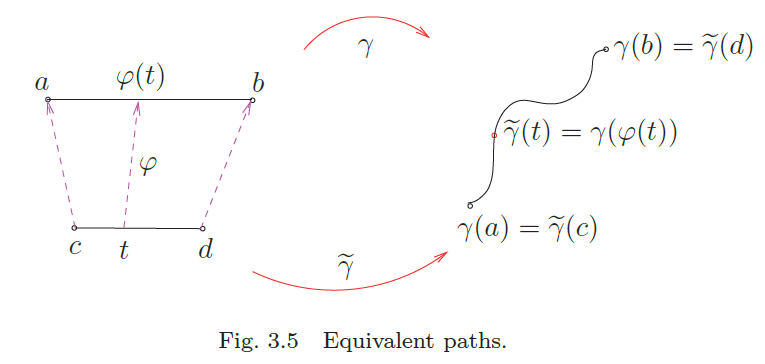
\includegraphics[width=0.7\textwidth]{./SaltChapter/fig-3-5}
\end{center}
\caption{동치 경로}
\label{fig-3-5}
\end{figure}
이제 다음 결과를 보일 수 있다.

{\bf 동치 경로에 대한 적분결과는 동일하다:}
연쇄법칙에 의해 다음이 성립한다.
\begin{align*}
\int_{\tilde\gamma}f(z)dz
&= \int_c^d f(\tilde\gamma(t))\tilde\gamma'(t)dt
= \int_c^d f(\gamma(\varphi(t)))\gamma'(\varphi(t)) \varphi'(t)dt \\
&\stackrel{(\tau=\varphi(t))}=
\int_a^b f(\gamma(\tau))\gamma'(\tau)d\tau
= \int_{\gamma}f(z)dz.
\end{align*}
특히, 주어진 $\gamma:[a,b]\to\mathbb C$에 대하여
$\varphi: [0,1]\to [a,b]$를 다음과 같이 정의하자.
\[
\varphi(t) = (1-t)a + tb, \quad t\in [a,b].
\]
그러면 $\varphi$는 연속미분가능하고,
$\varphi(0)=a$, $\varphi(1)=b$이다.
따라서 $c:=0$, $d:=1$로 두고 위의 결과를 적용하면,
$\tilde\gamma : [0,1]\to\mathbb C$를
$\tilde\gamma = \gamma\circ\varphi$라 정의하여
다음을 얻는다.
\[
\int_{\tilde\gamma} f(z)dz = \int_\gamma f(z)dz.
\]
결론적으로, 경로적분과 관련하여
매끄러운 곡선은 $[0,1]$에서 매개화된 것으로 간주해도 일반성을 잃지 않는다.

{\bf 조각적으로 매끄러운 경로에 대한 경로적분:}
경로의 정의를 ``꺽인 점''을 갖는 경로까지 확장해보자.
점 $c_1, \ldots, c_n$가
\[
a<c_1 < \cdots <c_n <b
\]
를 만족하고 $\gamma$가 구간 $[a,c_1], [c_1,c_2], \ldots, [c_{n_1}, c_n], [c_n,b]$ 각각에서
연속미분가능할 때,
경로 $\gamma:[a,b]\to\mathbb C$가 {\bf 조각적으로 매끄러운 경로 또는 곡선}이라 한다.
이러한 경로에서의 적분은 다음과 같이 정의한다.
\begin{align*}
\int_\gamma f(z)dz
&:= \int_a^{c_1} f(\gamma(t))\gamma'(t)dt + \int_{c_1}^{c_2} f(\gamma(t))\gamma'(t)dt
+ \cdots \\
&\quad \quad + \int_{c_{n-1}}^{c_n} f(\gamma(t))\gamma'(t)dt 
+ \int_{c_n}^b f(\gamma(t))\gamma'(t)dt.
\end{align*}

\begin{salt_example} \label{example-3-3}
$0$부터 $1+i$까지의 경로 $\tilde\gamma$가 다음과 같이 정의된다고 하자.
\[
\tilde\gamma(t) = \begin{cases}
t, & t\in[0,1], \\
1+(t-1)i, t\in (1,2].
\end{cases}
\]
그림 \ref{fig-3-6}을 보자.
\begin{figure}[!h]
\begin{center}
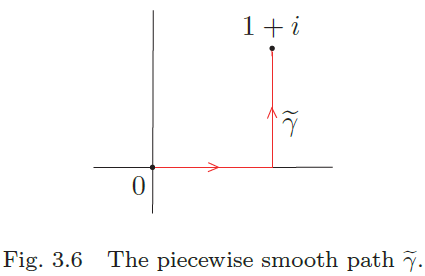
\includegraphics[width=0.4\textwidth]{./SaltChapter/fig-3-6}
\end{center}
\caption{조각적으로 매끄러운 경로 $\tilde\gamma$}
\label{fig-3-6}
\end{figure}
그러면
\begin{align*}
\int_{\tilde\gamma} \bar z dz 
&= \int_0^1 \bar t \,1\,dt
+ \int_1^2 \overline{(1+(t-1)i)}\,i\, dt
= \int_0^t t\,dt + \int_1^2 (1-(t-1)i)i\,dt \\
&= \int_0^1 t\,dt + \int_1^2 (i+(t-1))dt \\
&= \dfrac12 + i + \dfrac{4-1}2 - 1 = 1+ i.
\end{align*}
\end{salt_example}

예제 \ref{example-3-2}와 \ref{example-3-3}에서 얻은 계산결과를 돌아보자.
피적분함수는 같고($z\to\bar z$로 복소해석함수는 아니다),
그림 \ref{fig-3-7}과 같이
동일한 양끝점 $0$과 $1+i$를 연결하는 두 경로 $\gamma$와 $\tilde\gamma$에 대하여
\begin{figure}[!h]
\begin{center}
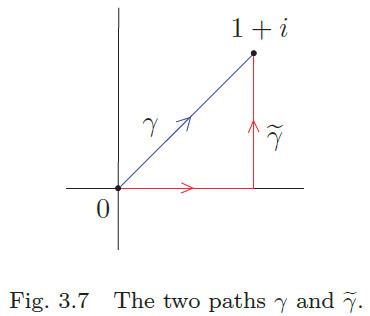
\includegraphics[width=0.4\textwidth]{./SaltChapter/fig-3-7}
\end{center}
\caption{두 경로 $\gamma$와 $\tilde\gamma$}
\label{fig-3-7}
\end{figure}
다른 적분 결과를 얻었다.
\[
\int_\gamma \bar z dz = 1 \ne 1+i = \int_{\tilde\gamma}\bar z dz.
\]
따라서 복소해석함수가 아닌 피적분함수 $z\to\bar z$는 경로에 따라 적분결과가 다르다.
경로적분의 정의를 보면
선택한 길에 따라 계산된 경로적분의 값이 다를 것으로 기대되기 때문에
뜻밖의 결과가 아니다.
이 장에서 중요한 목표는 
점 $z$에서 $w$까지 연결하는 두 경로 사이의 영역에서 복소해석적인 함수에 대해서는
두 경로를 따라 적분한 결과는 동일함을 보이는 것이다.
이 결과는 코시 적분 정리라 불리는 복소해석학의 핵심 결과로 이어진다.

\begin{salt_example} \label{example-3-4}
앞의 예제 \ref{example-3-2}와   \ref{example-3-3}에서 정의한
경로 $\gamma$, $\tilde\gamma$를 생각하자.
이번에는 피적분함수로 복소해석함수가 아니었던 $z\mapsto\bar z$ 대신 
전해석함수 $z$를 사용하자. 그러면,
\begin{align*}
\int_\gamma z dz 
&= \int_0^1 (1+i)t(1+i)dt = \int_0^1 2it\,dt = i \text{ 이고,} \\
\int_{\tilde\gamma} z dz
&= \int_0^1 t\cdot1\, dt + \int_1^2 (1+(t-1)i)i\, dt \\
&= \int_0^1 t\, dt + \int_1^2 (i-(t-1))dt
= \dfrac 12 - \dfrac12 + i = i  \text{ 이므로}
\end{align*}
경로 $\gamma$와 경로 $\tilde\gamma$를 따른  경로적분값이 동일하다.
\hfill $\diamondsuit$
\end{salt_example}

\begin{salt_exercise} \label{ex-3-3}
원 $|z|=2$를 따라 반시계방향의 한바퀴 도는 경로로 다음 함수를 적분하라.
\begin{itemize}
\item[(1)] $z+\bar z$
\item[(2)] $z^2-2z+3$
\item[(3)] $xy$ ($z=x+iy$, $x,y\in\mathbb R$)
\end{itemize}
\end{salt_exercise}


\begin{salt_exercise} \label{ex-3-4}
다음 경로 $\gamma$를 따라 적분 $\dint_\gamma \Re(z)dz$를 계산하라.
\begin{itemize}
\item[(1)] $0$에서 $1+i$까지 직선으로 연결한 선분
\item[(2)] 중심이 $i$이고 반지름이 $1$인 원을 따라 $0$부터 $1+i$까지 연결한 원호
\item[(3)] 포물선 $y=x^2$위에서 $x=0$부터 $x=1$까지 $0$과 $1+i$를 연결한 곡선
\end{itemize}
\end{salt_exercise}

\subsection{하나의 중요한 적분계산}

여기서 간단하지만 매우 중요한 경로적분 하나를 계산할 것인데
이 적분은 앞으로 계속 반복하여 다시 돌아볼 예정이다.
하나의 규칙을 정하자: 이 책 전체를 통하여 특별히 언급하지 않으면
$z_0$를 중심으로 반지름이 $r>0$인 원을 따라 반시계방향으로 도는 경로
$C: [0, 2\pi] \to \mathbb C$는 $C(t) = z_0 + r\exp(it)$, $t\in[0,2\pi]$로 정의한다
(따라서 한바퀴만 돈다). 그림 \ref{fig-3-8}을 참고하라.
\begin{figure}[!h]
\begin{center}
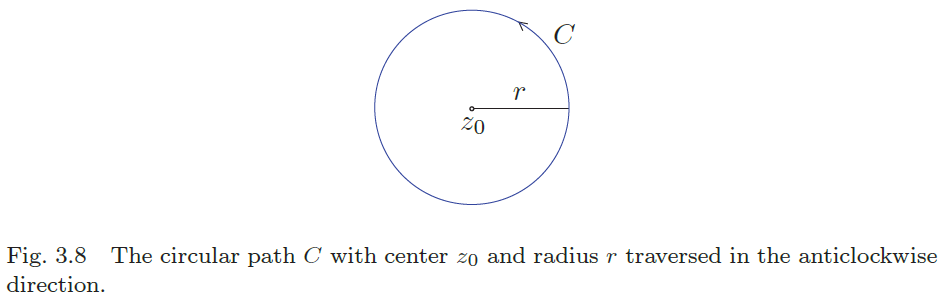
\includegraphics[width=0.9\textwidth]{./SaltChapter/fig-3-8}
\end{center}
\caption{$z_0$를 중심으로 반지름이 $r$인 원을 반시계방향으로 도는 경로 $C$}
\label{fig-3-8}
\end{figure}

이제 적분 $\int_C (z-z_0)^n dz$ ($n\in\mathbb Z$)를 계산하자.
나중에 이 계산이 매우 유용한 것으로 입증될 것이다.

\begin{salt_theorem} \label{thm-3-1}
$C$를 중심이 $z_0$이고 반지름 $r>0$인 원을 반시계방향으로 도는 경로라 하자.
그러면,
\[
\int_C (z-z_0)^n dz = \begin{cases}
2\pi i, & n=-1,\\
0, & n\ne -1.
\end{cases}
\]
여기서 적분값은 $r$에 무관함을 알 수 있다.
\end{salt_theorem}

{\bf 증명}

경로는 $C(t) = z_0 + r\exp(it) = z_0 + r\cos t + it\sin t$ ($t\in[0,2\pi]$)이므로
미분은 $C'(t) = -r\sin t + ir\cos t = ir(\cos t + i\sin t) = ir\exp(it)$ ($t\in[0,2\pi]$)이다.
두 가지 경우의 적분을 각각 계산하면,

\begin{itemize}
\item[$1^\circ$] $n=-1$일 때,
\begin{align*}
\int_C (z-z_0)^n dz
&= \int_C (z-z_0)^{-1} dz = \int_0^{2\pi} \dfrac1{r\exp(it)}\cdot ir \exp(it)dt \\
&= \int_0^{2\pi} i dt  = 2\pi i.
\end{align*}
\item[$2^\circ$] $n\ne -1$일 때,
\begin{align*}
\int_C (z-z_0)^n dz
&= \int_0^{2\pi} r^n \exp(nit) \cdot ir \exp(it)dt \\
&= \int_0^{2\pi} ir^{n+1} \exp(i(n+1)t)dt \\
&= -r^{n+1} \int_0^{2\pi} \sin((n+1)t)dt + 
ir^{n+1} \int_0^{2\pi} \cos((n+1)t)dt \\
&= 0+0 = 0.
\end{align*}
\end{itemize}
이로써 증명이 완성된다.
\hfill $\square$

우리는 나중에 이 결과가 의미심장한 결과를 갖는다는 것을 보게 될 것이다.
예를 들어, 
중심이 $z_0$, 안쪽 반지름이 $r$, 바깥쪽 반지름이 $R$인 
원환 $\mathbb A := \{ z\in\mathbb C \,:\, r<|z-z_0|<R \}$에 정의된
$f$가 $z$에 대하여 ``정수 지수를 갖는 항으로 된 급수전개''를 가진다고 가정하자 
(그 의미가 무엇이든).
\[
f(z) = \sum_{n\in\mathbb Z} a_n (z-z_0)^n, \quad z\in \mathbb A.
\]
이 (무한) 합의 정확한 의미는 나중에 알아보기로 하고
지금은 단지 유한 합 (유한개의 $a_n$을 제외하고는 모두 $0$되는)이라 생각해도 된다.
그러면  양변에 $(z-z_0)^{-(m+1)}$ ($m\in \mathbb Z$)을 곱하여 
\[
\dfrac{f(z)}{(z-z_0)^{m+1}} = \sum_{n\in\mathbb Z} a_n (z-z_0)^{n-m-1}
\]
을 얻게 되므로
\[
\dfrac1{2\pi i} \int_C \frac{f(z)}{(z-z_0)^{m+1}} dz
= \sum_{n\in\mathbb Z} a_n \int_C (z-z_0)^{n-m-1}dz = a_m.
\]
여기서 우리는 $C$을 따르는 경로적분과 합의 순서를 바꿀 수 있다고 가정했는데,
유한 합의 경우는 다음 절에서 적분의 정의로부터 가능함을 보일 것이다.
무한 합의 경우는 나중에 정확한 의미를 만들어 가겠지만 근본적으로는
제안한 계산 방식대로 작동한다.
궁극적으로는 계수들이 경로적분으로 표현될 수 있다는 것을 의미하며,
우리는 나중에 원환에 정의된 복소해석함수는 항상 이러한 급수 표현을 갖는다는 것을
보일 예정이다.

\begin{salt_exercise} \label{ex-3-5}
$C$를 중심이 $0$이고 반지름이 $1$인 원을 반시계방향으로 도는 경로라고 하자.
$0\le k \le n$에 대하여 다음이 성립함을 보여라.
\[
{n \choose k} = \dfrac1{2\pi i}\int_C \dfrac{(1+z)^n}{z^{k+1}} dz.
\]
\end{salt_exercise}

\section{경로적분의 성질}

이 절에서는 경로적분의 몇가지 유용한 성질을 살펴볼 것이다.
다음 정리는 경로적분의 정의로부터 직접 얻을 수 있다.

\begin{salt_prop} \label{prop-3-1}
복소수 $\mathbb C$의 영역 $D$에 대하여
$\gamma: [a,b] \to D$가 조각적으로 연속인 경로라고 하자.
그러면 다음이 성립한다.
\begin{itemize}
\item[(1)] 연속함수 $f,g : D \to \mathbb C$에 대하여,
\[
\int_\gamma (f+g)(z) dz = \int_\gamma f(z)dz + \int_\gamma g(z)dz.
\]
\item[(2)] 연속함수 $f : D \to \mathbb C$와 상수 $\alpha\in\mathbb C$에 대하여,
\[
\int_\gamma  (\alpha f)(z)dz = \alpha \int_\gamma f(z)dz.
\]
\end{itemize}
\end{salt_prop}
$C(D;\mathbb C)$를
$D$에 정의된 연속인 복소함수의 (점별 연산에 대한) $\mathbb C$상의 벡터공간이라 하자.
\footnote{역주: 점별연산이란 $f$, $g$의 합 $h:=f+g$을 $h(z):=f(z)+g(z)$로 정의함을 뜻한다}
그러면 위 결과는 $D$에 속하는 조각적으로 매끄러운 경로 $\gamma$는
$C(D;\mathbb C)$에서 $\mathbb C$로의 선형변환을 유도함을 의미한다.
\footnote{역주: $T: C(D;\mathbb C) \to \mathbb C$가 선형변환이면
$T(f+g) = T(f)+T(g)$, $T(\alpha f) = T(f)$를 만족한다. }
즉,
\[
f \mapsto \int_\gamma f(z)dz : C(D;\mathbb C) \to \mathbb C.
\]

\begin{salt_exercise} \label{ex-3-6}
명제 \ref{prop-3-1}을 증명하라.
\end{salt_exercise}

{\bf 반대경로:}
영역 $D$에 매끄러운 경로 $\gamma: [a,b] \to D$가 
주어졌을 때, {\bf 반대경로} $-\gamma: [a,b] \to D$는
$(-\gamma)(t) = \gamma(a+b-t)$, $t\in[a,b]$로 정의한다.
그러면 $(-\gamma)(a) = \gamma(b)$, $(-\gamma)(b) = \gamma(a)$이다.
따라서 $-\gamma$는 $\gamma$의 끝점에서 시작하고,
$\gamma$의 시작점에서 끝나는 경로이며,
$\gamma$와 동일한 길을 반대 방향으로 이동한다.
그림 \ref{fig-3-9}를 보라.
\begin{figure}[!h]
\begin{center}
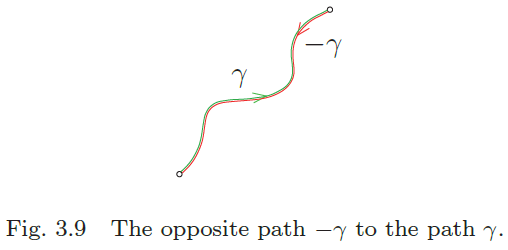
\includegraphics[width=0.5\textwidth]{./SaltChapter/fig-3-9}
\end{center}
\caption{경로 $\gamma$의 반대경로 $-\gamma$}
\label{fig-3-9}
\end{figure}

그런데 왜 반대경로를 $-\gamma$라고 쓸까?
그 이유는 다음과 같다.

\begin{salt_prop} \label{prop-3-2}
$\gamma: [a,b] \to D$가 영역 $D$의 매끄러운 경로이고
$f:D\to\mathbb C$가 연속함수라고 하자. 그러면
\[
\int_{-\gamma} f(z)dz = - \int_\gamma f(z)dz.
\]
\end{salt_prop}

{\bf 증명}

\begin{align*}
\int_{-\gamma} f(z)dz
&= \int_a^b f((-\gamma)(t))\cdot (-\gamma)'(t)dt \\
&= \int_a^b f(\gamma(a+b-t))\cdot (\gamma'(a+b-t))\cdot(-1)dt \\
& \stackrel{(\tau=a+b-t)}=
\int_b^a f(\gamma(\tau))\cdot \gamma'(\tau)d\tau 
= - \int_a^b f(\gamma(\tau))\cdot \gamma'(\tau)d\tau \\
&= - \int_\gamma f(z)dz.
\end{align*}
\hfill $\square$

\begin{salt_exercise} \label{ex-3-7}
$\gamma: [a,b] \to D$가 영역 $D$의 매끄러운 경로일 때,
$-(-\gamma) = \gamma$임을 보여라.
\end{salt_exercise}

{\bf  경로의 결합:}
영역 $D$에 대하여, 두 경로
\begin{align*}
\gamma_1 &: [a_1, b_1] \to D, \\
\gamma_2 &: [a_2, b_2] \to D
\end{align*}
가 다음을 만족한다고 하자.
\[
\gamma_1(b_1) = \gamma_2(a_2)
\]
(그러면 $\gamma_2$는 $\gamma_1$의 끝점에서 시작한다.)
경로의 결합 $\gamma_1+\gamma_2: [a_1, b_1+b_2-a_2] \to D$를
다음과 같이 정의한다.
\[
(\gamma_1+\gamma_2)(t) = \begin{cases}
\gamma_1(t), & a_1\le t\le b_1, \\
\gamma_2(t-b_1+a_2), & b_1 \le t \le b_1+b_2-a_2.
\end{cases}
\]

\begin{figure}[!h]
\begin{center}
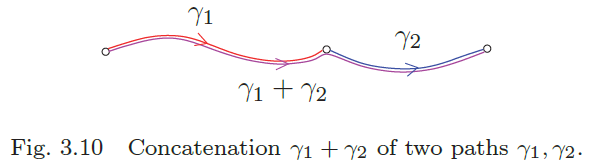
\includegraphics[width=0.6\textwidth]{./SaltChapter/fig-3-10}
\end{center}
\caption{두 경로 $\gamma_1$과  $\gamma_2$의 결합 $\gamma_1 + \gamma_2$}
\label{fig-3-10}
\end{figure}

\begin{salt_prop} \label{prop-3-3}
$D$가 복소평면 $\mathbb C$의 영역이고
두 경로 $\gamma_1: [a_1,b_1] \to D$와 $\gamma_2: [a_2,b_2] \to D$가 
$\gamma_1(b_1) = \gamma_2(a_2)$를 만족한다고 하자.
그러면
\[
\int_{\gamma_1+\gamma_2} f(z)dz 
=\int_{\gamma_1} f(z)dz + \int_{\gamma_2} f(z)dz.
\]
\end{salt_prop}

{\bf 증명}
\begin{align*}
\int_{\gamma_1+\gamma_2} f(z)dz 
&= \int_{a_1}^{b_1+b_2-a_2} f((\gamma_1+\gamma_2)(t)) (\gamma_1+\gamma_2)'(t)dt\\
&= \int_{a_1}^{b_1} f((\gamma_1+\gamma_2)(t)) (\gamma_1+\gamma_2)'(t)dt\\
& \quad\quad 
+\int_{b_1}^{b_1+b_2-a_2} f((\gamma_1+\gamma_2)(t)) (\gamma_1+\gamma_2)'(t)dt\\
&= \int_{a_1}^{b_1} f(\gamma_1(t))\gamma_1'(t)dt \\
&\quad\quad 
+ \int_{b_1}^{b_1+b_2-a_2} f(\gamma_2(\tau-b_1+a_2))\gamma_2'(\tau-b_1+a_2)d\tau\\
&= \int_{\gamma_1} f(z)dz + \int_{a_2}^{b_2} f(\gamma_2(s)) \gamma_2'(s)ds 
\ (s=\tau-b_1+a_2) \\
&= \int_{\gamma_1} f(z)dz + \int_{\gamma_2} f(z)dz.
\end{align*}

\begin{salt_exercise} \label{ex-3-8}
$\gamma: [a,b] \to D$가 영역 $D$의 매끄러운 경로이고
$f:D\to\mathbb C$가 연속함수라고 하자. 다음을 증명하라.
\[
\dint_{\gamma+(-\gamma)} f(z)dz =0.
\]
\end{salt_exercise}

{\bf 유용한 판정식:}
이제 경로적분의 크기를 경로에서의 $|f|$의 크기, 경로의 길이의 관점에서
나타낸 부등식을 증명한다. 이 부등식은 향후 필수적인 것으로 입증될 것이다.

\begin{salt_prop} \label{prop-3-4}
\
\begin{itemize}
\item[(1)] $D$가 복소평면 $\mathbb C$의 영역이고,
\item[(2)]  $\gamma : [a,b] \to D$가 조각적으로 매끄러운 경로이고,
\item[(3)] $f:D\to\mathbb C$가 연속함수이면,
\end{itemize}
다음 부등식이 성립한다.
\begin{equation} \label{eq-3-3}
\left| \int_\gamma f(z)dz \right| 
\le \left( \max_{t\in[a,b]} |f(\gamma(t))| \right) 
\cdot (\gamma \text{의 길이}).
\end{equation}
$\gamma$의 길이는 
\[
\int_a^b \sqrt{ (x'(t))^2 + (y'(t))^2} dt
\]
로 주어지며 $x,y: [a,b] \to \mathbb R$는
경로 $\gamma$의 실수부와 허수부를 나타낸다.
그림 \ref{fig-3-11}을 보라.
\begin{figure}[!h]
\begin{center}
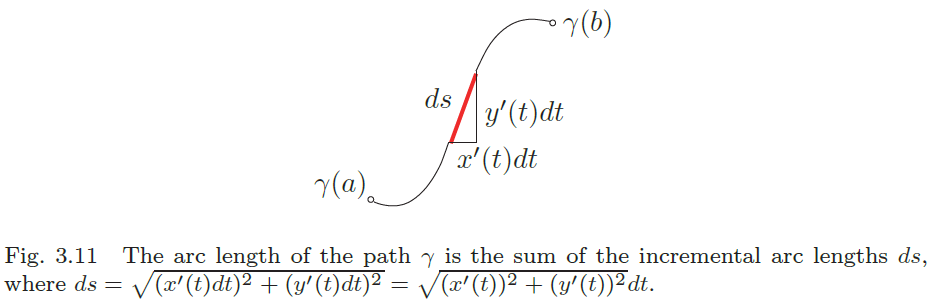
\includegraphics[width=0.9\textwidth]{./SaltChapter/fig-3-11}
\end{center}
\caption{경로 $\gamma$의 길이는 국소적인 곡선 길이 $ds$의 합이고,
$ds = \sqrt{(x'(t)dt)^2 + (y'(t)dt)^2} = \sqrt{(x'(t))^2 + (y'(t))^2}dt$이다.}
\label{fig-3-11}
\end{figure}
\end{salt_prop}

{\bf 증명}

우선 곡선 $\varphi : [a,b] \to \mathbb C$에 대하여 다음 부등식을 증명하자.
\[
\left| \int_a^b \varphi(t)dt \right|
\le \int_a^b |\varphi(t)|dt.
\]
이를 위해 $\dint_a^b \varphi(t) dt = r\cdot \exp(i\theta)$로 쓰자.
여기서 $r\ge 0$이고 $\theta \in (-\pi, \pi]$이다.
그러면,
\begin{align*}
\left| \int_a^b \varphi(t)dt \right|
&= r = \exp(-i\theta)\cdot r \cdot \exp(i\theta) \\
&= \exp(-i\theta) \cdot \int_a^b \varphi(t)dt
= \int_a^b \exp(-i\theta) \cdot \varphi(t)dt \\
&= \int_a^b \Re(\exp(-i\theta)\cdot\varphi(t))dt
+ i \int_a^b \Im(\exp(-i\theta)\cdot\varphi(t))dt.
\end{align*}
그런데 좌변은 실수이므로, 우변의 허수부 적분은 $0$이 되어야 한다.
따라서 
\begin{align*}
\left| \int_a^b \varphi(t)dt \right|
&= \int_a^b \Re(\exp(-i\theta)\cdot\varphi(t))dt \\
&\le \int_a^b |\Re(\exp(-i\theta)\cdot\varphi(t))|dt \\
&\le \int_a^b | \exp(-i\theta) \cdot \varphi(t)| dt
= \int_a^b |\varphi(t)| dt. 
\end{align*}
$\varphi(t) := f(\gamma(t))\cdot \gamma'(t)$, $t\in[a,b]$라 두면
\begin{align*}
\left| \int_\gamma f(z)dz \right| 
&= \left| \int_a^b f(\gamma(t)) \gamma'(t) dt \right| \\
&\le \int_a^b |f(\gamma(t)) \gamma'(t)| dt
= \int_a^b |f(\gamma(t))| | \gamma'(t)| dt \\
&\le \left( \max_{t\in[a,b]} |f(\gamma(t))| \right) 
\int_a^b |\gamma'(t)|dt.
\end{align*}
실함수 $x, y$를 써서  $\gamma(t) = x(t) + iy(t)$라 쓰면
\[
\int_a^b |\gamma'(t)|dt 
= \int_a^b  \sqrt{ (x'(t))^2 + (y'(t))^2} dt
= \gamma \text{의 길이}
\]
가 되어 증명이 끝난다.
\hfill $\square$

\begin{salt_exercise} \label{ex-3-9}
$\gamma$가 $0$부터 $1+i$까지의 선분일 때,
적분 
\[
\int_\gamma z^2dz
\] 
의 절대값의 상한을 식 \eqref{eq-3-3}에 주어진 방법으로 계산하라.
또한, 직접 적분을 계산하고 절대값을 구하라.
\end{salt_exercise}

\begin{salt_exercise} \label{ex-3-10}
연습문제 \ref{ex-3-5}의 결과를 이용하여
$\displaystyle{2n \choose n} \le 4^n$을 보여라.
\end{salt_exercise}

\section{경로적분의 기본정리}

실함수에 대한 미적분학의 기본정리를 다시 보자.
\begin{salt_theorem}[미적분학의 기본정리] \label{thm-3-2}
$F:[a,b] \to \mathbb R$가 연속미분가능하고, 
$[a,b]$에서 $F'=:f$라 하면,
\[
\int_a^b f(x)dx = F(b) - F(a).
\]
\end{salt_theorem}

이 정리는 리만 적분의 계산을 용이하게 해주는 중요한 정리이다. 
실제로 함수가 어떤 함수의 도함수인 것을 안다면, 정적분을 쉽게 계산할 수 있다.
예를 들면,
\[
x^2 = \dfrac d{dx}\left( \dfrac{x^3}3\right) \text{을 이용하면, }
\int_a^b x^2 dx = \dfrac{b^3-a^3}3.
\]
유사하게,  함수 $f$가 복소해석함수의 미분이라면 
실함수에 대한 미적분학의 기본정리와 비슷한 다음 정리로부터 
경로적분
\[
\int_\gamma f(z)dz
\]
의 계산이 쉽게 얻어진다.

\begin{salt_theorem}[경로적분에 대한 미적분학의 기본정리] 
\footnote{실해석의 결과와 유사함을 강조하기 위해  정리의 이름에
``기본''이란 용어를 사용하였다. 하지만, 복소해석학에서는
그만큼 ``근본적( fundamental)''이진 않다. 
더 확실하게 근본적인 코시 적분정리를 곧 배우게 될 것이다. }
\label{thm-3-3}
\
\begin{itemize}
\item[(1)] $D$가 복소평면 $\mathbb C$의 영역이고,
\item[(2)] $\gamma : [a,b] \to D$가 조각적으로 매끄러운 경로이고,
\item[(3)] $f:D\to\mathbb C$가 $D$에서 연속함수이고,
\item[(4)] $F:D\to \mathbb C$가 $D$에서 $F'=f$를 만족하는 복소해석함수이면,
\end{itemize}
\[
\int_\gamma f(z)dz = F(\gamma(b)) - F(\gamma(a)).
\]
\end{salt_theorem}

이 정리가 어떤 도움을 줄까?
이제 우리는 어떤 경로적분들은 매우 쉽게 계산할 수 있다
(보통의 미적분에서와 마찬가지로).
아래 예제를 보자.

\begin{salt_example}\label{example-3-5}
$z\in\mathbb C$에 대하여
$\dfrac d{dz}\left( \dfrac{z^2}2\right)=z$이므로,
$0$부터 $1+i$까지의 임의의 경로 $\gamma$에 대한 적분은
\[
\int_\gamma z\, dz = \dfrac{(1+i)^2}2 - \dfrac{0^2}2 
= \dfrac{1+2i+i^2}2 = \dfrac{1+2i-1}2 = i
\]
가 되어 예제 \ref{example-3-4}와 같은 결과를 얻는다.
\hfill $\diamondsuit$
\end{salt_example}

앞의 예제에서 살펴본 바와 같이 
$D$에서 $f$가 ``부정적분'' 또는 ``원시함수''라 불리는 $F$를 가지면
\[
\int_\gamma f(z)dz = F(w) - F(z)
\]
은 $z$와 $w$를 잇는 경로 $\gamma$에 무관하다.

\begin{salt_example}\label{example-3-6}
모든 $\mathbb C$에 대하여 
$F'(z) = \bar z$를 만족하는 함수 $F:\mathbb C \to \mathbb C$는 없다.
실제로 예제 \ref{example-3-2}와 \ref{example-3-3}의 계산은
$0$부터 $1+i$까지의 적분이 경로에 의존적임을 보여준다.
\hfill $\diamondsuit$
\end{salt_example}

{\bf 증명} (정리 \ref{thm-3-3})

$z = x+iy\in D$ ($x,y\in \mathbb R$)에 대하여
실함수 $U$, $V$, $u$, $v$를 다음과 같이 정의하자.
\begin{align*}
F(x+iy) &= U(x,y) + iV(x,y), \\
f(x+iy) &= u(x,y) + iv(x,y).
\end{align*}
또한, $\gamma(t) = x(t) + iy(t)$ ($t\in[a,b]$)라고 하자.
여기서 $x$, $y$는 실함수이다.
그러면, 코시-리만 방정식에 의해
\begin{align*}
u(x,y) + iv(x,y) 
&= f(x+iy) = F'(x+iy) \\
&= \dfrac{\partial U}{\partial x}(x,y) + i \dfrac{\partial V}{\partial x}(x,y)
= \dfrac{\partial V}{\partial y}(x,y) - i \dfrac{\partial U}{\partial y}(x,y).
\end{align*}
위 식에 연쇄법칙을 적용하면,
\begin{align*}
\dfrac d{dt} U(x(t), y(t))
&= \dfrac{\partial U}{\partial x}(x(t),y(t))\cdot x'(t)
 + \dfrac{\partial U}{\partial y}(x(t),y(t))\cdot y'(t) \\
&= u(x(t),y(t))\cdot x'(t) - v(x(t),y(t))\cdot y'(t).
\end{align*}
비슷한 방법으로,
\begin{align*}
\dfrac d{dt} V(x(t), y(t))
&= \dfrac{\partial V}{\partial x}(x(t),y(t))\cdot x'(t)
 + \dfrac{\partial V}{\partial y}(x(t),y(t))\cdot y'(t) \\
&= v(x(t),y(t))\cdot x'(t) + u(x(t),y(t))\cdot y'(t).
\end{align*}
따라서,
\begin{align*}
\int_\gamma f(z)dz
&= \int_a^b f(\gamma(t))\gamma'(t)dt \\
&= \int_a^b \left( u(x(t), y(t)) + iv(x(t),y(t)) \right) (x'(t)+iy'(t))dt \\
&= \int_a^b \dfrac d{dt} U(x(t), y(t))dt + i \int_a^b \dfrac d{dt} V(x(t), y(t))dt \\
&= U(x(b), y(b)) - U(x(a), y(a)) + 
i\left( V(x(b), y(b)) - V(x(a), y(a)) \right) \\
&= F(\gamma(b)) - F(\gamma(a)).
\end{align*}
이로써 증명이 끝난다. \hfill $\square$

\begin{salt_exercise} \label{ex-3-11}
코시-리만 방정식을 이용하여
$\mathbb C$에 정의된 함수 $z \mapsto \bar z$는 원시함수(부정적분)를 
갖지 않음을 보여라.
\end{salt_exercise}

\begin{salt_exercise}[부분적분 공식] \label{ex-3-12}
영역 $D$에 정의된 복소해석함수 $f$, $g$의 미분
$f'$, $g'$이 $D$에서 연속이라고 하자.
영역 $D$ 내부의 경로 $\gamma$가 
점 $w\in D$에서 $z\in D$까지의  조각적으로 매끄러운 경로이면
다음 공식이 성립함을 보여라.
\[
\int_\gamma f(\zeta)g'(\zeta)d\zeta 
= f(z)g(z) - f(w)g(w) - \int_\gamma f'(\zeta)g(\zeta)d\zeta.
\]
\end{salt_exercise}

\begin{salt_exercise} \label{ex-3-13}
$-i$와 $i$를 잇는 임의의 경로 $\gamma$에 대하여
경로적분 $\dint_\gamma \cos z\, dz$를 계산하라.
\end{salt_exercise}

\begin{salt_definition} \label{def-3-2}
$\gamma:[a,b] \to \mathbb C$가
$\gamma(a)= \gamma(b)$를 만족하면 {\bf 닫힌경로}라고 한다.
\end{salt_definition}

\begin{figure*}[!h]
\begin{center}
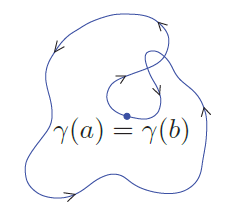
\includegraphics[width=0.25\textwidth]{./SaltChapter/fig-3-0-1}
\end{center}
\end{figure*}

\begin{salt_corollary} \label{coro-3-1}
\
\begin{itemize}
\item[(1)] $D$가 복소평면 $\mathbb C$의 영역이고,
\item[(2)] $\gamma : [a,b] \to D$가 조각적으로 매끄러운 {\bf 닫힌}경로이고,
\item[(3)] $f:D\to\mathbb C$가 $D$에서 연속함수이고,
\item[(4)] $F:D\to \mathbb C$가 $D$에서 $F'=f$를 만족하는 복소해석함수이면,
\end{itemize}
\ \ $\dint_\gamma f(z)dz = 0$.
\end{salt_corollary}

{\bf 증명}
$\gamma(b)=\gamma(a)$이므로,
$\dint_\gamma f(z)dz = F(\gamma(b)) - F(\gamma(a)) = 0$.
\hfill $\square$

\begin{salt_example}\label{example-3-7}
$m\in\mathbb Z\setminus \{0\}$, $z\in D:=\mathbb C \setminus\{0\}$
에 대하여, 
$\dfrac d{dz}\left( \dfrac{z^m}m\right) = z^{m-1}$이므로,
$D$의 임의의 닫힌경로 $\gamma$에 대하여
\[
\int_\gamma z^{m-1}dz = 0.
\]
$m=0$일 때는 어떻게 될까?
$z\in\tilde D:= \mathbb C \setminus (-\infty,0)$에서
$\Log' z = 1/z$이므로 $\tilde D$의 임의의 닫힌경로 $\tilde \gamma$에 대하여
\[
\int_{\tilde\gamma} \frac1z dz = 0
\]
임을 알고 있다. 하지만, 영역 $D$에서 $\dfrac 1z$는 부정적분을 갖지 않는다.
연습문제 \ref{ex-3-16}을 보라.
\end{salt_example}

\begin{salt_exercise} \label{ex-3-14}
경로적분의 기본정리를 이용하여 
$0$과 $a+ib$를 잇는 경로 $\gamma$에 대하여
다음 적분을 계산하라.
\[
\int_\gamma \exp z \, dz.
\]
$0$부터 $a+ib$까지 직선을 따라 매개변수 적분으로 계산한 결과와 동일함을 이용하여
다음 등식을 증명하라.
\[
\int_0^1 e^{ax}\cos(bx)\, dx = \dfrac{a(e^a\cos b - 1) + be^a\sin b}{a^2+b^2}.
\]
\end{salt_exercise}

\begin{salt_exercise} \label{ex-3-15}
$\exp z$와 원형 경로에 경로적분의 기본정리를 적용하여
모든 $r>0$에 대하여 다음 등식을 증명하라.
\[
\int_0^{2\pi} e^{r\cos\theta} \cos(r\sin\theta+\theta)d\theta = 0.
\]
\end{salt_exercise}

\begin{salt_exercise} \label{ex-3-16}
뚫린 평면 $\mathbb C\setminus \{0\}$에서 $1/z$는 부정적분을 갖지 않음을 보여라.
\end{salt_exercise}

\section{코시 적분정리}

이제 복소해석학의 중요 결과 중 하나인 코시 적분정리를 증명하고자 한다.

\begin{salt_theorem} [코시 적분정리] \label{thm-3-4}
\
\begin{itemize}
\item[(1)] $D$가 복소평면 $\mathbb C$의 영역이고,
\item[(2)] $f:D\to\mathbb C$가 $D$에서 복소해석적이고,
\item[(3)] 두 경로 $\gamma_0, \gamma_1 :[0,1]\to D$는  조각적으로 매끄러운 닫힌경로로
$D$-호모토픽(homotopic)이면,
\end{itemize}
\[
\int_{\gamma_0} f(z)dz = \int_{\gamma_1} f(z)dz.
\]
\end{salt_theorem}

더 진행하기에 앞서 정리의 의미를 이해해보자.
우선 $D$의 두 경로는 닫힌경로이다.
다음으로 두 닫힌경로가 $D$-호모토픽이라는 것은 무엇일까?
직관적으로 다음과 같은 의미를 가진다.
한 영역의 내부에 두 경로를 나타낸 그림 \ref{fig-3-12}를 보자.
$\gamma_0$를 따라 고무밴드를 위치시킨다고 상상하자.
$\gamma_0$가 $\gamma_1$과 $D$-호모토픽이려면
이 고무밴드를 변형하여 $\gamma_1$에 맞출 수 있어야 한다.
이 때, 중간과정에서 고무밴드의 위치는 반드시 영역 $D$의 내부에 머물러야 한다.
분명히 어떤 경우는 이 변형이 불가능할 수도 있다. 
예를 들면 영역에 구멍을 가진 경우가 그렇다.
그림 \ref{fig-3-12}의 오른쪽 그림을 보면 
영역 $D$를 뚫린 복소평면 $D=\mathbb C\setminus \{0\}$으로 정하면
영역의 두 경로가 $D$-호모토픽이 될 수 없다.

\begin{figure}[!h]
\begin{center}
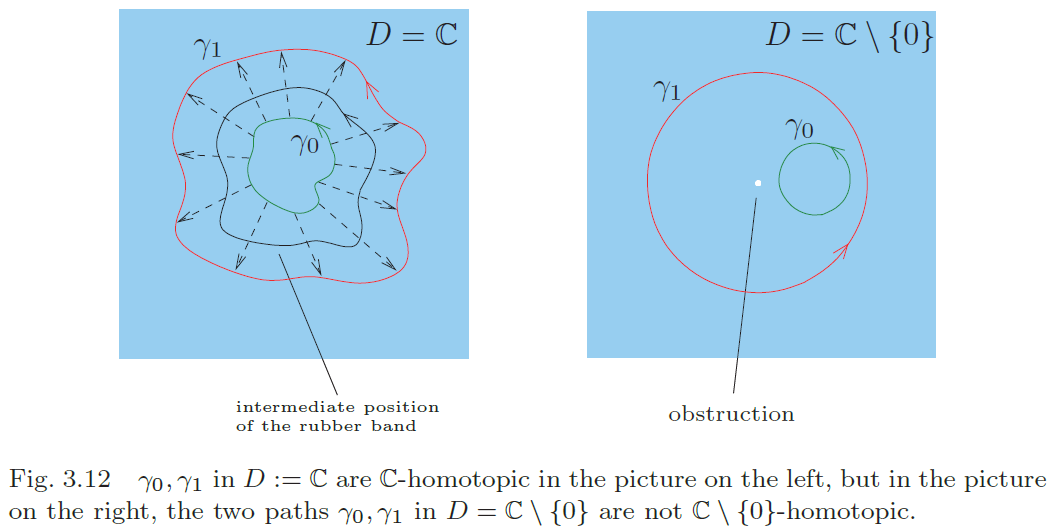
\includegraphics[width=0.9\textwidth]{./SaltChapter/fig-3-12}
\end{center}
\caption{왼쪽 그림에서 $D:=\mathbb C$의 경로 $\gamma_0, \gamma_1$은 $D$-호모토픽이다.
하지만, 오른쪽 그림에서 $D:=\mathbb C\setminus\{0\}$의 두 경로
$\gamma_0, \gamma_1$은 $\mathbb C\setminus\{0\}$-호모토픽이 아니다.}
\label{fig-3-12}
\end{figure}

이제 엄밀한 정의를 만들어보자.

\begin{salt_definition} \label{def-3-3}
$D$를 복소평면 $\mathbb C$의 영역,
$\gamma_0, \gamma_1 : [0,1] \to D$를 닫힌경로라고 하자.
다음 조건을 만족하는 연속함수 $H:[0,1]\times[0,1]\to D$가 존재하면
$\gamma_0$는 $\gamma_1$과 {\bf $D$-호모토픽}이라 한다.
\begin{itemize}
\item[(H1)] 모든 $t\in [0,1]$에 대하여, $H(t,0)=\gamma_0(t)$.
\item[(H2)] 모든 $t\in [0,1]$에 대하여, $H(t,1)=\gamma_1(t)$.
\item[(H3)] 모든 $s\in [0,1]$에 대하여, $H(0,s)=H(1,s)$.
\end{itemize}
\end{salt_definition}

$H$를 주어진 시각 $s$에 대하여
$[0,1]$에서 $D$로의 닫힌경로의 모임으로 간주할 수 있다.
시각 $s$에서 닫힌경로를 시각 $s$에서 고무밴드의 위치로 생각해도 된다.
초기에는 $s=0$이고, $H(\cdot, 0)$는 경로 $\gamma_0$가 되며,
마지막으로 $s=1$일 때, 경로 $\gamma_1$을 나타내는
$H(\cdot, 1)$가 된다.
여기까지는 조건 (H1)과 (H2)의 의미이다.
조건 (H3)로부터 주어진 시각 $s$에 대하여 중간 경로 
$\gamma_s:= H(\cdot, s)$도 닫힌경로임이다.
$H$의 연속성은 고무밴드가 끊어지지 않음을 보장하며
변형이 매끄럽게 이루어진다는 것을 의미한다.
아래 그림은 이를 표현한 것이다.

\begin{figure*}[!h]
\begin{center}
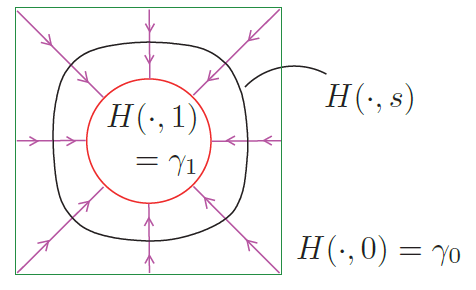
\includegraphics[width=0.35\textwidth]{./SaltChapter/fig-3-0-2}
\end{center}
\end{figure*}

\newpage  %===[salt: 페이지 조정]

\begin{salt_example} \label{example-2-8}
$D=\mathbb C$이고 원형 경로 $\gamma_0, \gamma_1 : [0,1] \to \mathbb C$가
$\gamma_0 = 4\exp(2\pi it)$와 $\gamma_1 = 2i+\exp(2\pi it)$ ($t\in[0,1]$)로 주어졌다고 하자.
그러면 $\gamma_0$는 $\gamma_1$과 $\mathbb C$-호모토픽이다.
실제로  $H$를 $\gamma_0(t)$와 $\gamma_1(t)$의 점에 대한 볼록결합으로 정의하면 된다.
그림 \ref{fig-3-8}을 참고하라.

\begin{figure*}[!h]
\begin{center}
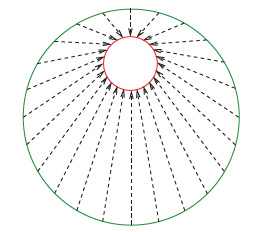
\includegraphics[width=0.3\textwidth]{./SaltChapter/fig-3-0-3}
\end{center}
\end{figure*}

$H:[0,1]\times [0,1] \to \mathbb C$를 
$H(t,s) = (1-s)\cdot \gamma_0(t) + s\cdot \gamma_1(t)
= (4-3s)\cdot \exp(2\pi it) + s\cdot 2i$ ($0\le t,s\le 1$)로 정의하자.
그러면 $H$가 연속임은 분명하며 다음이 성립한다.
\begin{itemize}
\item[(H1)] 모든 $t\in [0,1]$에 대하여, $H(t,0)= (4-0)\cdot \exp(2\pi it) + 0\cdot 2i = \gamma_0(t)$.
\item[(H2)] 모든 $t\in [0,1]$에 대하여, $H(t,1)= (4-3)\cdot \exp(2\pi it) + 1\cdot 2i = \gamma_1(t)$.
\item[(H3)] 모든 $s\in [0,1]$에 대하여, $H(0,s)= (4-3s)\cdot 1 + s\cdot 2i = H(1,s)$.
\end{itemize}
따라서 (H1), (H2), (H3)가 만족되므로 
$\gamma_0$는 $\gamma_1$과 $\mathbb C$-호모토픽이다.

한편, 이 경로들은 $\mathbb C\setminus \{0\}$-호모토픽은 아니다.
왜 그렇게 될까? 만일 $\mathbb C\setminus \{0\}$-호모토픽이라면
코시-적분정리에 의해 $\mathbb C\setminus \{0\}$에서 복소해석함수인
$1/z$의 두가지 경로적분이 같은 값을 가져야 한다. 하지만
\[
\int_{\gamma_0} \dfrac 1z dz = 2\pi i \ne 0 = \int_{\gamma_1} \dfrac 1z dz
\]
이므로 모순이다. 
$\mathbb C\setminus \{0\}$에서 $1/z$가 부정적분 $\Log z$을 가지므로,
마지막 등호는 경로적분의 기본정리로부터 얻어진다.
\hfill $\diamondsuit$
\end{salt_example}

\begin{salt_exercise} \label{ex-3-17}
$D$가 $\mathbb C$의 영역이라고 하자.
$D$의 모든 닫힌경로의 집합에서 $D$-호모토피는 동치관계임을 보여라.
특히, ``$\gamma_0$가 $\gamma_1$에 $D$-호모토픽하다''는 대신
``$\gamma_0$과 $\gamma_1$가 $D$-호모토픽하다''라고 쓸 수 있다.
\end{salt_exercise}

{\bf 증명} (정리 3.4)
호모토피 $H$가 두번 연속미분가능하다고 가정하자.
매끈함에 대한 이 조건을 생략해도 증명은 가능하다 ([Conway (1978)]을 보라). %==[salt] reference에 추가
하지만 증명이 복잡해진다. 
또한 두번 연속미분가능하다는 것이 강한 조건은 아니다.
앞으로 편미분의 순서를 바꿀 필요가 있을 때 이 조건을 사용할 것이다.
\[
\dfrac{\partial^2 H}{\partial s \partial t} =\dfrac{\partial^2 H}{\partial t \partial s}.
\]

{\bf 증명의 아이디어:}
시간 $s$에서의 중간 경로를 $\gamma_s := H(\cdot, s)$라 하고
다음과 같이 함수 $I(s)$를 정의하자.
\[
I(s) := \int_{\gamma_s} f(z)dz, \quad s\in [0,1].
\]
적분기호하에서 $s$에 대한 미분을 사용하여
\[
\dfrac d{ds} I(s) \equiv 0
\]
을 보임으로써 $s\mapsto I(s)$가 상수함수임을 증명할 것이다.
특히, 보이고자 하는 결론
\[
\int_{\gamma_0} f(z)dz = I(0) = I(1) = \int_{\gamma_1} f(z)dz
\]
가 성립한다.

\begin{align*}
\dfrac{dI}{ds}(s)
&= \dfrac d{ds} \int_{\gamma_s} f(z)dz 
= \dfrac d{ds} \int_0^1 f(H(t,s))\dfrac{\partial H}{\partial t}(t,s)dt \\
&= \int_0^1 \dfrac{\partial}{\partial s} \left( f(H(t,s))\dfrac{\partial H}{\partial t}(t,s) \right) dt \\
&= \int_0^1 \left(  f'(H(t,s))\dfrac{\partial H}{\partial s}(t,s)\dfrac{\partial H}{\partial t}(t,s)
+ f(H(t,s)) \textcolor{blue}{\dfrac{\partial^2H}{\partial s\partial t}(t,s)} \right) dt \\
&= \int_0^1 \left(  f'(H(t,s))\dfrac{\partial H}{\partial s}(t,s)\dfrac{\partial H}{\partial t}(t,s)
+ f(H(t,s)) \textcolor{blue}{\dfrac{\partial^2H}{\partial t\partial s}(t,s)} \right) dt \\
&= \int_0^1 \dfrac \partial{\partial t} \left( f(H(t,s)) \dfrac{\partial H}{\partial s}(t,s) \right) dt
\end{align*}
이므로 적분에 대한 기본정리에 의하여,
\begin{align*}
\dfrac{dI}{ds}(s)
&= \int_0^1 \dfrac \partial{\partial t} \left( f(H(t,s)) \dfrac{\partial H}{\partial s}(t,s) \right) dt \\
&= f(H(1,s))  \dfrac{\partial H}{\partial s}(1,s) - f(H(0,s)) \dfrac{\partial H}{\partial s}(0,s) \\
&= f(H(1,s)) \lim_{\sigma\to s} \dfrac{H(1,\sigma) - H(1,s)}{\sigma - s}
- f(H(0,s)) \lim_{\sigma\to s} \dfrac{H(0,\sigma) - H(0,s)}{\sigma - s} \\
&= f(H(1,s)) \lim_{\sigma\to s} \dfrac{H(1,\sigma) - H(1,s)}{\sigma - s}
- f(H(1,s)) \lim_{\sigma\to s} \dfrac{H(1,\sigma) - H(1,s)}{\sigma - s} \\
&=0.
\end{align*}
따라서 함수 $s\mapsto I(s): [0,1] \to \mathbb C$는 상수이고, 특히
다음이 성립한다.
\[
\int_{\gamma_0} f(z)dz = I(0) = I(1) = \int_{\gamma_1} f(z)dz.
\]
이로써 증명이 끝난다. 하지만 $f$가 복소해석함수라는 조건을 어디에서 사용했을까?
위 식의 세번째 줄에서 이 조건을 아래와 같이 사용했다.
\[
\dfrac\partial{\partial s}(f(H(t,s))) = f'(H(t,s))\cdot \dfrac{\partial H}{\partial s}(t,s).
\]
$f=u+iv$, $H=X+iY$라 하자 ($u,v,X,Y$는 실함수).
매개변수 $(t,s)$를 생략하고 식을 써보면 다음과 같다.
\begin{align*}
\dfrac\partial{\partial s}(f(H(t,s)))
&= \dfrac\partial{\partial s}(u(X,Y) + iv(X,Y)) \\
&= \dfrac{\partial u}{\partial x}(X,Y)\cdot \dfrac{\partial X}{\partial s}
+ \textcolor{red}{\dfrac{\partial u}{\partial y}(X,Y)}\cdot \dfrac{\partial Y}{\partial s} \\
&\quad\quad + i \left(
\dfrac{\partial v}{\partial x}(X,Y)\cdot \dfrac{\partial X}{\partial s}
+ \textcolor{blue}{\dfrac{\partial v}{\partial y}(X,Y)}\cdot \dfrac{\partial Y}{\partial s}
\right) \\
&= \dfrac{\partial u}{\partial x}(X,Y)\cdot \dfrac{\partial X}{\partial s}
- \textcolor{red}{\dfrac{\partial v}{\partial x}(X,Y)}\cdot \dfrac{\partial Y}{\partial s} \\
&\quad\quad + i \left(
\dfrac{\partial v}{\partial x}(X,Y)\cdot \dfrac{\partial X}{\partial s}
+ \textcolor{blue}{\dfrac{\partial u}{\partial x}(X,Y)}\cdot \dfrac{\partial Y}{\partial s}
\right) \\
&= \left( \dfrac{\partial u}{\partial x}(X,Y) + i \dfrac{\partial v}{\partial x}(X,Y) \right)
\cdot \left( \dfrac{\partial X}{\partial s} + i\dfrac{\partial Y}{\partial s} \right) \\
&= f'(X+iY)\cdot \dfrac \partial{\partial s} (X+iY)
= f'(H(t,s))\cdot \dfrac{\partial H}{\partial s}(t,s).
\end{align*}
주의깊은 독자는 적분기호하에서 미분할 때 $f'$이 연속이라고 가정했음을 알아챘을 것이다.
이 가정이 없어도 결과는 성립하지만 여기서 다루진 않을 것이다.
관심있는 독자는 [Conway (1978)] 등에서   %==[salt] reference에 추가
코시 적분정리의 완전한 증명을 찾아보기 바란다.
\hfill $\square$

\begin{salt_exercise} \label{ex-3-18}
$C$가 중심이 $0$이고 반지름 $1$인 원을 반시계방향으로 도는 원형 경로이면
\[
\int_C \dfrac 1z dz = 2\pi i
\]
임을 이미 알고 있다.
이제 $\pm 1$, $\pm i$를 꼭지점으로 하는 사각형을 따라 반시계방향으로 도는 경로 $S$를 생각하자.
그림을 그려서 $S$가 $C$와 $\mathbb C\setminus \{0\}$-호모토픽임을 확인하라.
매개변수 적분
\[
\int_S \dfrac 1z dz
\]
를 직접 계산하여 결과가 실제로 $2\pi i$가 됨을 확인하라.
\end{salt_exercise}

\begin{salt_exercise} \label{ex-3-19}
$a>0$, $b>0$이고, $E:[0,2\pi] \to \mathbb C$는 타원
\[
E(t) = a\cos t + ib\sin t, \quad t\in [0,2\pi]
\]
이라고 하자.
적분 $\dint_E \dfrac 1z dz$를 고려하여
$\dint_0^{2\pi} \dfrac 1{a^2(\cos \theta)^2 + b^2(\sin \theta)^2}d\theta = \dfrac{2\pi}{ab}$
임을 보여라.
\end{salt_exercise}

\subsection{특별한 경우: 단순연결 영역}

``퇴화된'' 단힌곡선으로 상수의 경우를 생각하자.
즉, $D$가 영역이고 $p\in D$일 때,
$\gamma_p:[0,1] \to D$가 모든 $t\in[0,1]$에 대하여 $\gamma_p(t)=p$인 경우이다.
그러면 $\gamma_p$는 $\gamma_p(0)=\gamma_p(1)$을 만족하므로 닫힌경로이다.
임의의 연속함수 $f:D\to\mathbb C$에 대하여, 적분
\[
\int_{\gamma_p} f(z)dz
\]
은 어떤 값을 가질까? 
모든 $t\in[0,1]$에 대하여 $\gamma_p'(t)=0$이므로 적분값은
$0$이 된다.
\[
\int_{\gamma_p} f(z)dz = \int_0^1 f(\gamma_p(t))\cdot \gamma_p'(t)dt = 0.
\]
이로부터 코시 적분정리의 특별하고 중요한 경우로
닫힌경로 $\gamma$가 한점(즉, 상수경로 $\gamma_p(t)=p$, $t\in[0,1]$)과 
$D$-호모토픽일 때를 생각할 수 있다.
이 경우  $\gamma$를  $D$-축약가능하다고 한다.
$\gamma$를 따라 고무밴드를 놓고 
중간단계에서 고무밴드가 $D$를 벗어나지 않도록 유지하며 수축시켜 한점으로 만들자. 
$D$-축약가능한 경로 $\gamma$ (즉, 한점 $p\in D$와 $D$-호모토픽인 경로)와
복소해석함수 $f:D \to \mathbb C$에 대하여
코시 적분정리로부터 다음 결과를 얻는다.
\[
\int_\gamma f(z) dz = \int_{\gamma_p} f(z) dz = 0.
\]
모든 닫힌경로가 $D$-축약가능한 영역을 {\bf 단순연결} 영역이라고 한다.

예를 들어 $\mathbb C$, $\mathbb D:=\{z\in\mathbb C\,:\, |z|<1\}$,
$\mathbb C\setminus(-\infty,0]$는 모두 단순연결 영역이다.
앞의 두 예에서 영역에 속하는 임의의 점 $p$를 잡으면 호모토피를 다음과 같이 만들 수 있다.
\[
H(t,s) := (1-s)\gamma(t) = sp, \quad t,s\in[0,1].
\]
$\mathbb C\setminus(-\infty,0]$의 경우는
임의의 경로 $\gamma: [0,1] \to D$에 대하여
점 $p$를 양수로 잡으면 (예를 들어 $p=1$) 위와 같은 $H$를 만들 수 있다.
위의 예는 공통적으로 ``구멍''을 갖지 않는다는 점에 주목하자.
한편 구멍을 갖는 영역은 단순연결 영역이 아니다. 예를 들어
뚫린 복소평면 $\mathbb C\setminus \{0\}$은 단순연결이 아니다.
중심이 $0$이고 반지름 $r$인 원을 반시계방향으로 한바퀴 도는 원형 경로에 대하여
\[
\int_C \dfrac 1z dz = 2\pi i
\]
이다. 그런데 $C$가 뚫린 복소평면의 어떤 한점으로 
$\mathbb C\setminus \{0\}$-축약가능하다면
코시 적분정리에 의하여
\[
\int_C \dfrac 1z dz = 0
\]
이 되어여 한다.
따라서 $C$는 $\mathbb C\setminus \{0\}$의 한점으로 $\mathbb C\setminus \{0\}$-축약가능한 
경로가 아니며 $\mathbb C\setminus \{0\}$는 단순연결 영역이 아니다.
유사하게 원환
\[
\{ z\in\mathbb C \,:\,  1<|z|<2 \}
\]
가 단순연결이 아님을 보일 수 있다.
그림 \ref{fig-3-13}을 보자.
구멍의 방해는 명면을 뚫고 나오는 못 또는 기둥으로 생각할 수 있으며,
이는 구멍을 둘러싸고 있는 고무밴드가 평면을 떠나지 않으면서
한점으로 축소되는 것을 막는다.
\begin{figure}[!h]
\begin{center}
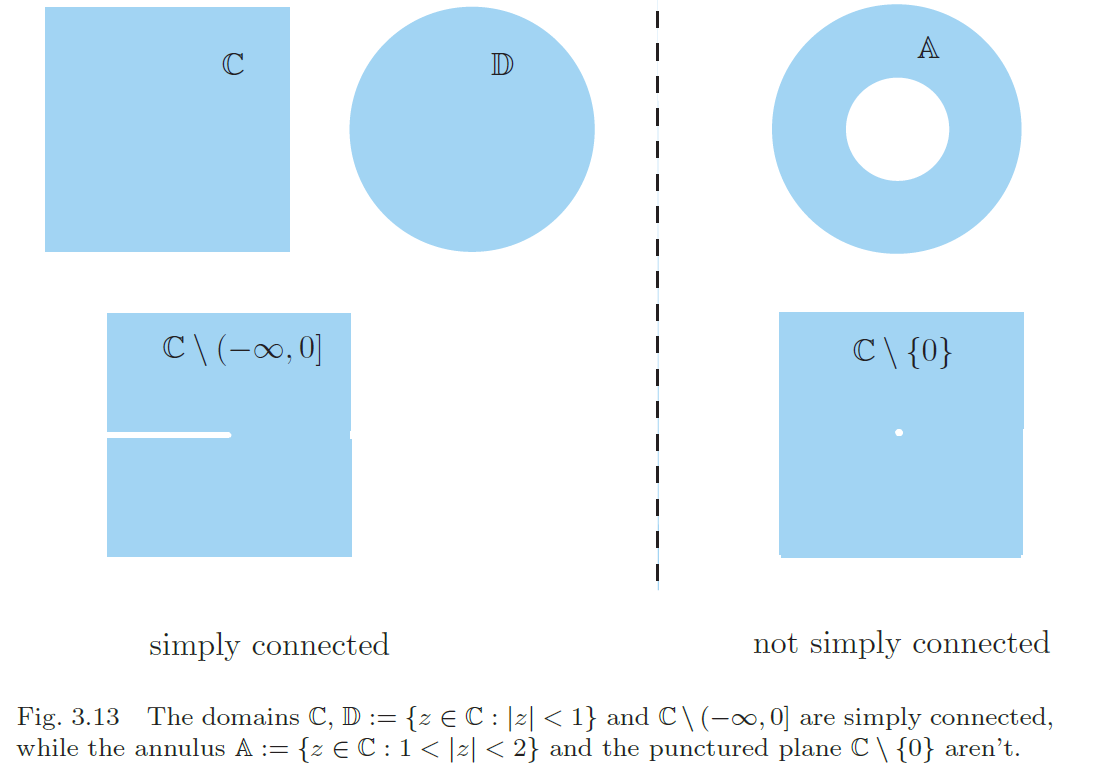
\includegraphics[width=0.9\textwidth]{./SaltChapter/fig-3-13}
\end{center}
\caption{$\mathbb C$, $\mathbb D:=\{z\in\mathbb C\,:\, |z|<1\}$,
$\mathbb C\setminus(-\infty,0]$는 모두 단순연결 영역이지만,
원환 $\mathbb A:= \{ z\in\mathbb C \,:\,  1<|z|<2 \}$와 
뚫린 복소평면 $\mathbb C\setminus \{0\}$는 아니다.}
\label{fig-3-13}
\end{figure}

다음은 코시 적분정리의 따름정리이다.

\begin{salt_corollary} \label{coro-3-2}
\
\begin{itemize}
\item[(1)] $D$가 단순연결 영역이고,
\item[(2)] $\gamma$는 영역 $D$에서 조각적으로 매끄러운 닫힌경로이고,
\item[(3)] $f:D\to\mathbb C$는 $D$에서 복소해석적이면,
\end{itemize}
\[
\int_\gamma f(z)dz = 0.
\]
\end{salt_corollary}

이 따름정리가 코시 적분정리로 불리기도 한다.

\begin{salt_example} \label{example-3-9}
$\exp$가 전해석함수이고, $\mathbb C$가 단순연결 영역이므로
임임의 닫힌경로 $\gamma$에 대하여
\[
\int_\gamma \exp z \, dz = 0.
\]
실제로 임의의 전해석함수 $f$와 임의의 닫힌경로 $\gamma$에 대하여, $\dint_\gamma f(z)dz=0$이다.
\hfill $\diamondsuit$
\end{salt_example}

$D$가 단순연결 영역이 아닌 경우에도 복소미분가능한 함수 $f:D\to \mathbb C$가
영역 $D$의 임의의 닫힌경로 $\gamma$에 대하여
\[
\dint_\gamma f(z)dz=0
\]
를 만족할 수 있다.
예를 들면 $D=\mathbb C\setminus \{0\}$, $f:=1/z^2$이면,
$1/z^2$은 $\mathbb C\setminus \{0\}$에서 부정적분을 가지므로
\[
\dfrac d{dz}\left(- \dfrac 1z\right) = \dfrac1{z^2}, \quad z\in \mathbb C\setminus \{0\},
\]
뚫린 복소평면의 임의의 닫힌경로 $\gamma$에 대하여
\[
\int_\gamma \dfrac 1{z^2}dz=0.
\]

\begin{salt_exercise} \label{ex-3-20}
$|z|=3$을 따라 반시계방향으로 도는 원형 경로를 따라 다음 함수의 적분을 구하라.
\begin{itemize}
\item[(1)] $\Log (z-4i)$.
\item[(2)] $\dfrac1{z-1}$.
\item[(3)] $i^{z-3}$의 주치.
\end{itemize}
\end{salt_exercise}

\begin{salt_exercise}[경로의 회전수] \label{ex-3-21}
$\gamma:[0,1]\to\mathbb C$가 $0$을 지나지 않는
매끄러운 닫힌경로라고 가정하자. ($0$에 대한) $\gamma$의 {\bf 회전수}를 
다음과 같이 정의한다.
\[
w(\gamma) := \dfrac1{2\pi i}\int_\gamma \dfrac 1z dz
= \dfrac1{2\pi i}\int_0^1 \dfrac{\gamma'(t)}{\gamma(t)}dt.
\]
\begin{itemize}
\item[(1)] $\exp(2\pi ia)=1$일 필요충분조건이 $a\in\mathbb Z$임을 이용하여,
$w(\gamma)\in\mathbb Z$임을 다음 과정으로 증명하라.
함수 $\varphi:[0,1] \to\mathbb C$를 
\[
\varphi(t) = \exp\left( \int_0^t \dfrac{\gamma'(s)}{\gamma(s)}ds\right),
\quad t\in[0,1]
\]
로 정의하자.  $w(\gamma)\in\mathbb Z$를 증명하려면
$\varphi(1)=1$을 보이면 충분하다.
이를 위해, $\varphi'(t)$를 계산하여 $\varphi/\gamma$가 $[0,1]$에서 상수임을 증명하라.
이 사실로부터 $\varphi(1)=1$이라는 결론을 얻을 수 있다.
\item[(2)] $\Gamma_1(t)=\exp(2\pi it)$ ($t\in[0,1]$)로 주어진 경로 $\Gamma_1:[0,1]\to\mathbb C$의
회전수를 계산하라.
\item[(3)] $\gamma_1, \gamma_2:[0,1]\to\mathbb C$가 $0$을 지나지 않는
매끄러운 닫힌경로라 하자. 두 경로의 곱 $\gamma_1\cdot\gamma_2$을
점별 곱으로 정의하면, $w(\gamma_1\cdot\gamma_2) = w(\gamma_1)+w(\gamma_2)$임을
증명하라.
\item[(4)] $m\in \mathbb N$이라 하자. 
$\Gamma_m(t)=\exp(2\pi imt)$ ($t\in[0,1]$)로 주어진 경로 $\Gamma_m:[0,1]\to\mathbb C$의
회전수를 계산하라.
\item[(5)] 회전수 함수 $\gamma \mapsto w(\gamma)$는
``국소적으로 상수함수''임을 보여라.
즉, $\gamma_0:[0,1]\to\mathbb C\setminus\{0\}$가 매끄러운 닫힌경로이면,
$\|\gamma -\gamma_0\|_\infty := \max\{ |\gamma(t) - \gamma_0(t)| \,:\, t\in[0,1]\}<\delta$를
만족하는 모든 닫힌경로 $\gamma:[0,1]\to\mathbb C\setminus\{0\}$에 대하여
$w(\gamma) = w(\gamma_0)$가 되도록 하는 $\delta>0$가 존재한다.
(다시 말하면, 곡선의 집합에 균등 위상(uniform topology)을 설정하고
$\mathbb Z$에 이산 위상(discrete topology)을  설정하면,
$\gamma \mapsto w(\gamma)$는 연속함수이다)
\end{itemize}
\end{salt_exercise}

\subsection{복소해석함수가 아닌 경우는 어떻게 될까?}

이제 $f$가 복소해석함수라는 가정을 생략하면 코시 적분정리가 만족되지 않을 수 있음을 강조하고자 한다.
복소해석함수가 아님을 잘 알고있는 켤레복소수 함수 $z\mapsto \bar z$에 정리를 적용하면
어떻게 되는지 살펴보자.
$0$을 둘러싸는 닫힌경로 $\gamma$를 따라 적분하는 경우,
$\bar z$를 $\gamma$를 따라 경로적분한 결과는 $\gamma$로 둘러싸인 영역의 넓이와 
같음을 보일 것이다.
당연히 넓이는 경로 $\gamma$의 모양에 의존하므로 $\mathbb C$-호모토픽한 두 경로로
둘러싸인 영역의 넓이는 다르다(단지 다른 반지름을 가진 두개의 동심원을 상상해보면 충분하다).
엄밀한 증명을 대신하여
아래 그림과 같이 특정 영역에 대한 타당한 설명만 제공하고자 한다 . %==[salt] 의역함

\begin{figure*}[!h]
\begin{center}
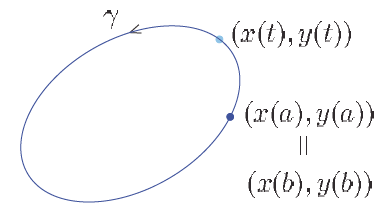
\includegraphics[width=0.25\textwidth]{./SaltChapter/fig-3-0-4}
\end{center}
\end{figure*}

매끄러운 경로 $\gamma: [a,b] \to \mathbb C$에 대하여
\begin{align*}
\int_\gamma \bar z\, dz
&= \int_a^b (x(t)-iy(t))(x'(t)+iy'(t))dt \\
&= \int_a^b x(t)x'(t)+y(t)y'(t) + i((x(t)y'(t)-y(t)x'(t))dt \\
&= \dfrac{(x(b))^2-(x(a))^2 + (y(b))^2 - (y(a))^2}2\
+ i \int_a^b ((x(t)y'(t)-y(t)x'(t))dt \\
&= 0 + i \int_a^b ((x(t)y'(t)-y(t)x'(t))dt.
\end{align*}

\begin{figure}[!h]
\begin{center}
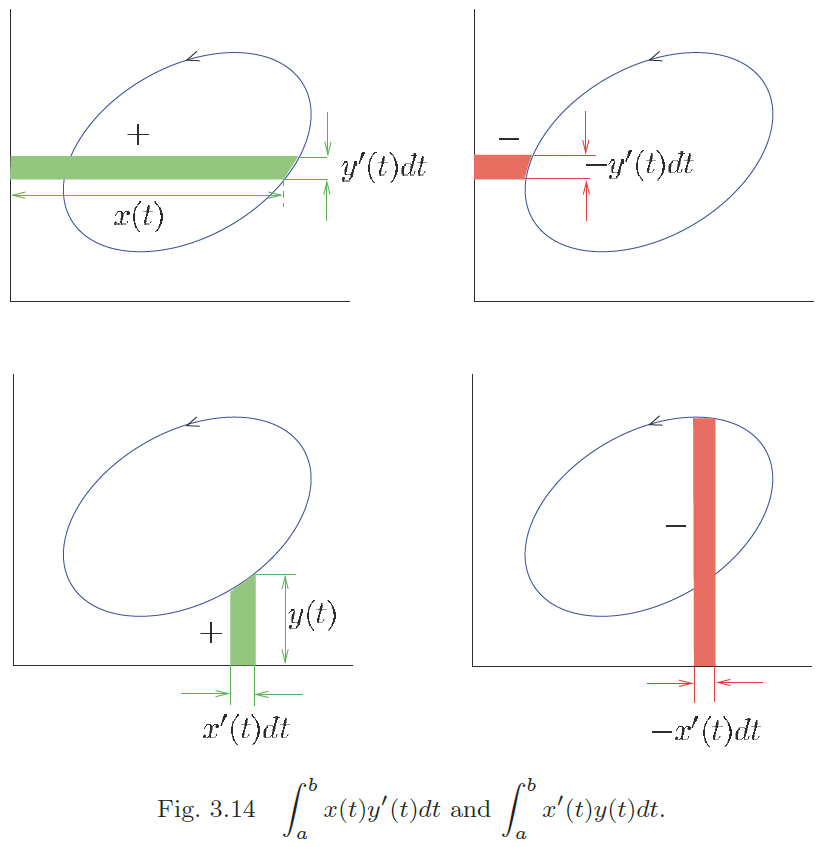
\includegraphics[width=0.8\textwidth]{./SaltChapter/fig-3-14}
\end{center}
\caption{$\dint_a^b x(t)y'(t)dt$와 $\dint_a^b x'(t)y(t)dt$
}
\label{fig-3-14}
\end{figure}

그림 \ref{fig-3-14}를 보면,  
위쪽 두 그림에서
\[
\int_a^b x(t)y'(t)dt = (\gamma\text{로 둘러싸인 영역의 넓이})
\]
이고, 아래 두 그림에서 다음 식을 얻는다.
\[
\int_a^b x'(t)y(t)dt = - (\gamma\text{로 둘러싸인 영역의 넓이})
\]
종합하면 $\dint_\gamma \bar z\, dz = i\dint_a^b ((x(t)y'(t)-y(t)x'(t))dt
= 2i\cdot (\gamma\text{로 둘러싸인 영역의 넓이})$.
따라서 복소해석함수에 대한 코시 적분정리와 달리
이와 같이 복소해석함수가 아닌 경우는 닫힌경로를 따라 적분한 결과가
$0$이 아니며, $\bar z$의 경우는 영역의 넓이와 관련이 있다!

\begin{salt_exercise} \label{ex-3-22}
반지름 $r$의 동전이 고정된 반지름 $R$의  더 큰 동전에 외접하며 구른다고 가정하자.
이 때, 구르는 동전의 둘레에 있는 한점이 그리는 경로를 에피사이클로이드라 부른다.
어떤 자연수 $n\in\mathbb N$에 대하여 $R=nr$를 만족하면 닫힌경로가 얻어진다.
그림 \ref{ex-3-22}를 보라.

\begin{figure}[!h]
\begin{center}
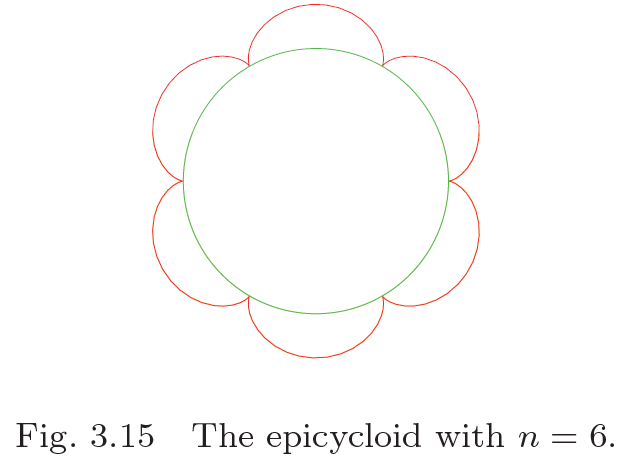
\includegraphics[width=0.4\textwidth]{./SaltChapter/fig-3-15}
\end{center}
\caption{$n=6$인 에피사이클로이드(epicycloid) 곡선}
\label{fig-3-15}
\end{figure}

\begin{itemize}
\item[(1)] 고정된 동전의 중점을 원점으로 설정하면,
에피사이클로이드는 다음과 같은 매개변수방정식으로 쓸 수 있음을 보여라.
\[
 z(t) = r((n+1)\exp(it) - \exp(i(n+1)t)), \quad t\in [0,2\pi].
\]
\item[(2)] 에피사이클로이드를 따라 함수 $\bar z$의 적분을 계산함으로써
에피사이클로이드로 둘러싸인 영역의 넓이가 $\pi r^2(n+1)(n+2)$가 됨을 보여라.
\end{itemize}
\end{salt_exercise}

이 장의 나머지 부분에서는
코시 적분정리에서 파생된 다양한 결과를 배울 예정이다.
특히, 다음과 같은 주제를 다룬다.

\begin{itemize}
\item[(1)] 단순연결 영역에서 모든 복소해석함수는 부정적분(원시함수)을 갖는다.
\item[(2)] 복소해석함수는 무한번 미분가능하다.
\item[(3)] 유계인 전해석함수는 상수함수 뿐이다 (리우비유 정리).  \\
(이 결과를 이용하여 대수학의 기본정리를 증명한다)
\item[(4)] 모레라 정리라 불리는 코시 적분정리의 역의 일종이 성립힌다.
\end{itemize}

\section{부정적분의 존재성}

단순연결 영역에서 모든 복소해석함수는 어떤 복소해석함수의 도함수가 됨을 증명하자.

\begin{salt_theorem} \label{thm-3-5}
\
\begin{itemize}
\item[(1)] $D$가 단순연결 영역이고,
\item[(2)] $f:D\to\mathbb C$가 복소해석함수이면,
\end{itemize}
모든 $z\in D$에 대하여 $F'(z) = f(z)$를 만족하는 
복소해석함수 $F:D\to\mathbb C$가 존재한다.
\end{salt_theorem}

{\bf 증명}

한점 $p\in D$를 고정하고 $F:D\to\mathbb C$를 다음과 같이 정의하자.
\[
F(z) = \int_{\gamma_z} f(\zeta)d\zeta, \quad z\in D,
\]
여기서 $\gamma_z$는 $p$와 $z$를 잇는 $D$ 내부의 경로이다.
$F$는 잘 정의된 함수인가? 즉, $F(z)$가 $p$에서 $z$까지의 경로에
의존하지 않고 정의되는가?
$\tilde \gamma_z$를 $p$와 $z$를 잇는 $D$의 다른 경로라 하면,
$\gamma_z - \tilde\gamma_z$는 단순연결 영역 $D$의
매끄러운 닫힌경로이다. 그림 \ref{fig-3-16}을 참고하자.

\begin{figure}[!h]
\begin{center}
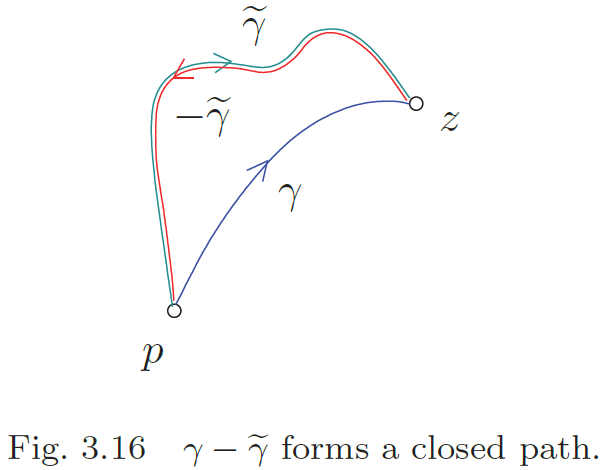
\includegraphics[width=0.4\textwidth]{./SaltChapter/fig-3-16}
\end{center}
\caption{$\gamma - \tilde \gamma$가 만드는 닫힌경로}
\label{fig-3-16}
\end{figure}

코시 적분정리로부터 
\[
0 = \int_{\gamma_z - \tilde\gamma_z}f(z)dz 
= \int_{\gamma_z} f(\zeta)d\zeta 
- \int_{\tilde\gamma_z} f(\zeta)d\zeta 
\]
이므로 $\dint_{\gamma_z}f(\zeta)d\zeta = \dint_{\tilde\gamma_z} f(\zeta)d\zeta$가 되어 
$F$가 잘 정의된다.

다음 단계로 $D$에서 $F'=f$를 만족하여 $F$가 복소해석함수가 됨을 증명하자.
$D$에서 $f$가 복소해석함수이므로
연속함수도 된다. 
따라서 주어진 점 $z\in D$에서 임의의 $\epsilon>0$에 대하여
대응하는 $\delta>0$가 존재하여
$|w-z|<\delta$이면 $|f(w)-f(z)|<\epsilon$을 만족한다.
이제 $w$를 $0<|w-z|<\delta$가 되도록 잡으면
\[
\dfrac{F(w)-F(z)}{w-z} = \dfrac1{w-z} \left(
\int_{\gamma_w} f(\zeta)d\zeta - \int_{\gamma_z} f(\zeta)d\zeta \right).
\]

$\gamma_{zw}$를 $z$와 $w$를 잇는 선분이라 하면,
경로 $\gamma_z$, $\gamma_{zw}$, $-\gamma_w$를 연접하면
닫힌경로가 되고 코시 적분정리를 적용하면 다음을 얻는다.
\[
0 = \int_{\gamma_z  + \gamma_{zw} - \gamma_w} f(\zeta)d\zeta
= \int_{\gamma_z} f(\zeta)d\zeta + \int_{\gamma_zw} f(\zeta)d\zeta
- \int_{\gamma_w} f(\zeta)d\zeta.
\]
\begin{figure*}[h!]
\begin{center}
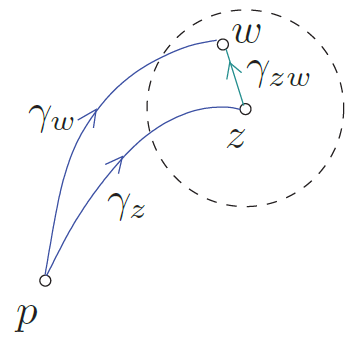
\includegraphics[width=0.25\textwidth]{./SaltChapter/fig-3-0-5}
\end{center}
\end{figure*}

경로적분의 기본정리로부터
\[
\int_{\gamma_{zw}} 1d\zeta = \int_{\gamma_{zw}} \zeta'd\zeta = w - z
\]
이므로
\begin{align*}
\dfrac{F(w)-F(z)}{w-z} - f(z)
&= \dfrac1{w-z} \int_{\gamma_{zw}} f(\zeta)d\zeta 
- \dfrac1{w-z} \int_{\gamma_{zw}} f(z)d\zeta \\
&= \dfrac1{w-z} \int_{\gamma_{zw}} (f(\zeta) - f(z)) d\zeta
\end{align*}
이고
\begin{align*}
\left| \dfrac{F(w)-F(z)}{w-z} - f(z) \right|
&= \left| \dfrac1{w-z} \int_{\gamma_{zw}} (f(\zeta) - f(z)) d\zeta \right| \\
&= \dfrac1{|w-z|} \left| \int_{\gamma_{zw}} (f(\zeta) - f(z)) d\zeta \right| \\
&= \dfrac1{|w-z|} \left( \max_{\zeta\in\gamma_{zw}} |f(\zeta) - f(z)| \right) \cdot
(\text{length of }\gamma_{zw}) \\
&< \dfrac1{|w-z|} \epsilon |w-z| = \epsilon.
\end{align*}
따라서 $F'(z) = f(z)$가 되어 $F$는 복소해석함수이다.
\hfill $\square$

\begin{salt_remark} \label{remark-3-2}
단순연결 영역에서 복소해석함수 $f$의 부정적분은 상수를 무시하면 유일하게 결정된다.
실제로 $F$와 $\tilde F$가 모두 $f$의 부정적분이라고 하면
$D$에서 $F' = f = \tilde F'$가 되어
\[
\dfrac d{dz} (F- \tilde F) = F' - \tilde F' = f - f = 0 \quad (D\text{에서}).
\]
연습문제 \ref{ex-2-13}에 의해
$F-\tilde F= C$를 만족하는 상수 $C$가 존재한다.
즉, $D$에서 $F = \tilde F + C$이다.
\end{salt_remark}

\begin{salt_example} \label{example-3-10}
$\exp(-z^2)$은 전해석함수이다.
따라서 모든 $z\in\mathbb C$에 대하여 $F'(z)= \exp(-z^2)$을 만족하는 함수 $F$가 존재한다
(하지만 우리는 $F$를 기본함수를 이용하여 나타내지는 못한다).
한가지 부정적분은 다음식으로 쓸 수 있다.
\[
\tilde F(z) = \int_{\gamma_z} e^{-\zeta^2} d\zeta, \quad (z\in\mathbb C),
\]
여기서 $\gamma_z$는 $0$과 $z$를 잇는 선분으로 정하자.
그러면 특히 실수 $x$에 대하여,
\[
\tilde F(x) = \int_0^x e^{-\xi^2} d\xi,
\]
이고 이 값은 (다른 부정적분도 마찬가지로) 기본함수로 표현할 수 없다.
\hfill $\diamondsuit$
\end{salt_example}

\begin{salt_exercise} \label{ex-3-23}
영역 $D$가 주어졌다고 하자.
$f$가 $D$에서 복소해석함수이고 $D$에서 $F'=f$를 만족하는
복소해석함수 $F$가 존재하지 않는다면,
$D$는 단순연결 영역이 될 수 없음을 알 수 있다.
$D$와 $f$의 구체적인 예를 제시하라.
\end{salt_exercise}

\begin{salt_corollary} \label{coro-3-3}
\
\begin{itemize}
\item[(1)] $D$가 단순연결 영역이고,
\item[(2)] $f:D\to\mathbb C$가 복소해석함수이고,
\item[(3)] $\gamma :[a,b] \to D$와 $\tilde\gamma :[c,d] \to D$가 
같은 시작점과 끝점을 갖는 매끄러운 경로이면
(즉, $\gamma(a) = \tilde\gamma(c)$이고 $\gamma(c) = \tilde\gamma(d)$이다),
\end{itemize}
\[
\int_\gamma f(z) dz = \int_{\tilde\gamma} f(z)dz.
\]
\end{salt_corollary}

\begin{figure*}[h!]
\begin{center}
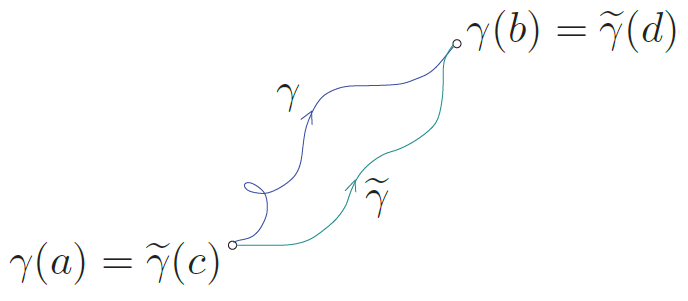
\includegraphics[width=0.4\textwidth]{./SaltChapter/fig-3-0-6}
\end{center}
\end{figure*}

{\bf 증명}
$f$가 부정적분 $F$를 가지므로
\[
\int_\gamma f(z) dz = F(\gamma(b)) - F(\gamma(a))
= F(\tilde\gamma(d)) - F(\tilde\gamma(c))
= \int_{\tilde\gamma} f(z)dz.
\]

\section{코시 적분공식}

이제 코시 적분공식이라 불리는 결과를 학습할 예정인데,
개요를 말하자면, 자신과는 교차하지 않는 닫힌경로 $\gamma$와
$\gamma$ 내부에서 복소해석함수인 $f$에 대하여,
$\gamma$ 내부 임의의 점에서 함수 $f$의 값은
$\gamma$위에서의 함수값으로 결정된다!
이는 복소해석함수의 ``엄밀성''을 보여주는 예이다.

다음 장에서 좀 더 일반적인 코시 적분공식을 공부할 계획인데,
$\gamma$ 내부의 점에서 $f$의 모든 미분은 
$\gamma$위에서의 함수값으로 표현된다.
따라서 이 장에서는 일반화된 결과 중 ``$n=0$인 경우''의 기본 결과만을 고려한다.

\begin{salt_theorem}[원형 경로에 대한 코시 적분공식] \label{thm-3-6}
\
\begin{itemize}
\item[(1)] $D$가 영역이고,
\item[(2)] $f:D\to\mathbb C$가 복소해석함수이고,
\item[(3)] $r>0$, $z_0\in D$, 
$\Delta := \{ z\in \mathbb C\,:\, |z-z_0| \le r\} \subset D$를 만족하면,
\end{itemize}
\[
f(w) = \dfrac1{2\pi i} \int_{C_r} \dfrac{f(z)}{z-w} dz, 
\quad |w-z_0| <r,
\]
여기서 $C_r$은 $C_r(t) = z_0 + r\exp(it)$, $t\in [0,2\pi]$로 
정의된, 중심이 $z_0$이고 반지름이 $r>0$인 
원을 반시계방향으로 도는 경로이다.

\begin{figure*}[h!]
\begin{center}
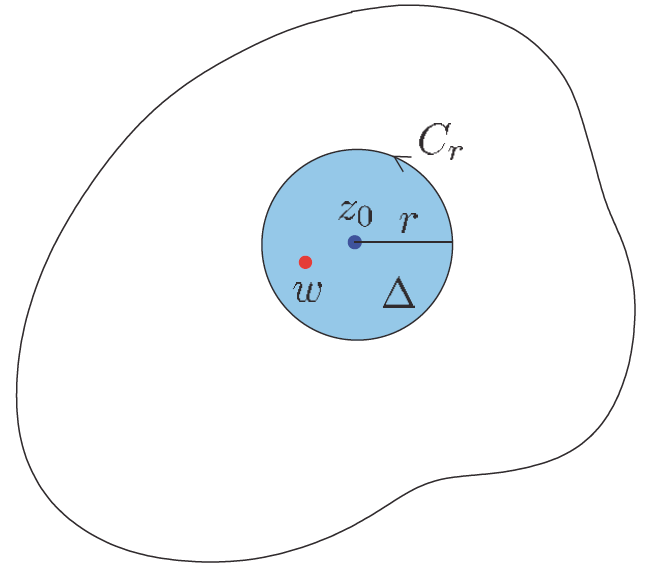
\includegraphics[width=0.4\textwidth]{./SaltChapter/fig-3-0-7}
\end{center}
\end{figure*}
\end{salt_theorem}

이 결과를 증명하기 위해 나중에 유용하게 사용될 다음 계산기법을 먼저 보이도록 하자.

\begin{salt_prop} \label{prop-3-5}
\
\begin{itemize}
\item[(1)] $D$가 영역이고, $z_0\in D$,
\item[(2)] $f:D\to\mathbb C$가 \textcolor{red}{$D\setminus \{z_0\}$}에서 복소해석함수이고,
\textcolor{red}{$D$에서 연속이고},
\item[(3)] $r>0$, 
$\Delta := \{ z\in \mathbb C\,:\, |z-z_0| \le r\}$가 $D$에 포함되면,
\end{itemize}
\[
f(z_0) = \dfrac1{2\pi i} \int_{C_r} \dfrac{f(z)}{z-z_0} dz, 
\]
여기서 $C_r$은 $C_r(t) = z_0 + r\exp(it)$, $t\in [0,2\pi]$로 
정의된, 중심이 $z_0$이고 반지름이 $r>0$인 
원을 반시계방향으로 도는 경로이다.
\end{salt_prop}

{\bf 증명}
$\epsilon>0$이라 하자.
그러면 $\delta>0$ ($r$보다 작게 잡는다)가 존재하여
$0<|z-z_0|\le \delta$이면 $|f(z) - f(z_0)|<\epsilon$을 만족한다.
중심이 $z_0$, 반지름이 $\delta$인 원을 반시계방향으로 도는 원형 경로 $C_\delta$를 생각하자.
$C_\delta$와 $C_r$은 $D\setminus\{z_0\}$-호모토픽임을 쉽게 알 수 있다.

\begin{figure*}[h!]
\begin{center}
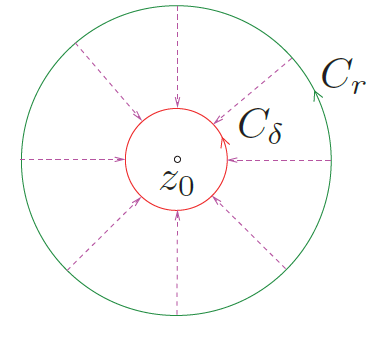
\includegraphics[width=0.3\textwidth]{./SaltChapter/fig-3-0-8}
\end{center}
\end{figure*}

실제로 호모토피 $H$는 $C_r$과  $C_\delta$ 위의 점들에 대한 볼록결합으로 얻을 수 있다.
\[
H(\cdot, s) := (1-s)C_r(\cdot) + sC_\delta(\cdot), 
\quad s\in [0,1].
\]
그러면 코시 적분정리에 의해 
\[
\int_{c_r} \dfrac{f(z)}{z-z_0}dz = \int_{c_\delta} \dfrac{f(z)}{z-z_0}dz
\]
이므로
\begin{align*}
\left| \dfrac1{2\pi i} \int_{c_r} \dfrac{f(z)}{z-z_0}dz - f(z_0) \right|
&= \left|  \dfrac1{2\pi i}\int_{c_\delta} \dfrac{f(z)}{z-z_0}dz - 
f(z_0)  \dfrac1{2\pi i} \int_{c_\delta} \dfrac{1}{z-z_0}dz \right| \\
&= \left|  \dfrac1{2\pi i}\int_{c_\delta} \dfrac{f(z)-f(z_0)}{z-z_0}dz \right| \\
&\le \left( \max_{z\in C_\delta} \dfrac{|f(z)-f(z_0)|}{|z-z_0|}  \right) \cdot 2\pi\delta \\
&< \dfrac \epsilon{2\pi \delta} \cdot 2\pi \delta = \epsilon.
\end{align*}
$\epsilon>0$은 임의로 작게 잡을 수 있으므로 증명이 끝난다.
\hfill $\square$

이로부터 다음 따름정리를 바로 얻을 수 있다.

\begin{salt_corollary} \label{coro-3-4}
\
\begin{itemize}
\item[(1)] $D$가 영역이고, 
\item[(2)] $f:D\to\mathbb C$가 $D$에서 복소해석함수이고,
\item[(3)] $r>0$, $z_0\in D$, 
$\Delta := \{ z\in \mathbb C\,:\, |z-z_0| \le r\} \subset D$를 만족하면,
\end{itemize}
\[
f(z_0) = \dfrac1{2\pi i} \int_{C_r} \dfrac{f(z)}{z-z_0} dz,
\]
여기서 $C_r$은 $C_r(t) = z_0 + r\exp(it)$, $t\in [0,2\pi]$로 
정의된, 중심이 $z_0$이고 반지름이 $r>0$인 
원을 반시계방향으로 도는 경로이다.
\end{salt_corollary}

이제 코시 적분공식의 기본형인 정리 \ref{thm-3-6}을 증명하자.
따름정리 \ref{coro-3-4}와 달리
$w$는 중심 $z_0$, 반지름 $r$인 원 내부의 {\bf 임의의} 점이며,
따름정리와 같이 반드시 중심 $z_0$일 필요가 없다.

{\bf 증명} (정리 \ref{thm-3-6})

$w$를 $|w-z_0| <r$을 만족하는 점이라 하자.
$\delta>0$를 충분히 작게 잡아 
중심이 $w$, 반지름이 $\delta$인 원형 경로 $C_\delta$가 $C_r$의 내부에 포함되도록 한다.
그러면 $C_r$과 $C_\delta$는 $D\setminus\{w\}$-호모토픽임을
예제 \ref{example-3-8}과 같은 방법으로 보일 수 있다.

\begin{figure*}[h!]
\begin{center}
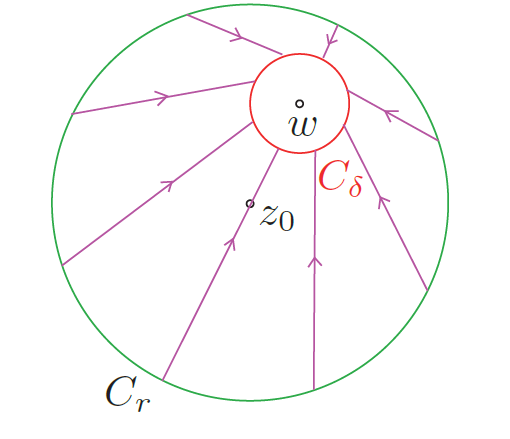
\includegraphics[width=0.3\textwidth]{./SaltChapter/fig-3-0-9}
\end{center}
\end{figure*}
$D\setminus\{w\}$에서
\[
\dfrac{f(\cdot)}{\cdot - w}
\]
가 복소미분가능함수이므로 코시 적분정리로부터 아래 두번째 등호가 성립한다.
\[
f(w) = \dfrac 1{2\pi i} \int_{C_\delta} \dfrac{f(z)}{z-w}dz
= \dfrac 1{2\pi i} \int_{C_r} \dfrac{f(z)}{z-w}dz.
\]
이로써 증명이 끝난다. \hfill $\square$

\begin{salt_exercise} \label{ex-3-24}
$0<a<1$이고, $\gamma$는 중심이 $0$인 단위원을 반시계방향으로 도는 경로일 때,
다음을 증명하라.
\[
\int_\gamma \dfrac{i}{(z-a)(az-1)}dz = \int_0^{2\pi} \dfrac 1{1+a^2-2a\cos t}dt.
\]
코시 적분공식을 이용하여 
$\dint_0^{2\pi} \dfrac 1{1+a^2-2a\cos t}dt = \dfrac{2\pi}{1-a^2}$을 유도하라.
\end{salt_exercise}

\begin{salt_exercise} \label{ex-3-25}
아래 빈 칸을 채워라.
\begin{itemize}
\item[(1)] $\dint_\gamma \dfrac{\exp z}{z-1}dz = \underline{\quad\quad\quad\quad}$,
단, $\gamma$는 $|z|=2$를 반시계방향으로 도는 원형 경로이다.
\item[(2)] $\dint_\gamma \dfrac{z^2+1}{z^2-1}dz = \underline{\quad\quad\quad\quad}$,
단, $\gamma$는 $|z-1|=1$를 반시계방향으로 도는 원형 경로이다.
\item[(3)] $\dint_\gamma \dfrac{z^2+1}{z^2-1}dz = \underline{\quad\quad\quad\quad}$,
단, $\gamma$는 $|z-i|=1$를 반시계방향으로 도는 원형 경로이다.
\item[(4)] $\dint_\gamma \dfrac{z^2+1}{z^2-1}dz = \underline{\quad\quad\quad\quad}$,
단, $\gamma$는 $|z+1|=1$를 반시계방향으로 도는 원형 경로이다.
\item[(5)] $\dint_\gamma \dfrac{z^2+1}{z^2-1}dz = \underline{\quad\quad\quad\quad}$,
단, $\gamma$는 $|z|=3$를 반시계방향으로 도는 원형 경로이다.
\end{itemize}
\end{salt_exercise}

\begin{salt_exercise} \label{ex-3-26}
영역 $\{ z\in \mathbb C\,:\, 0<|z|<1\}$에서
함수 $z\mapsto \dfrac1{z(1-z^2)}$은 부정적분을 갖는가?
\end{salt_exercise}

\begin{salt_corollary} [일반 경로에 대한 코시 적분공식] \label{coro-3-5}
\
\begin{itemize}
\item[(1)] $D$가 영역이고, 
\item[(2)] $f:D\to\mathbb C$가 $D$에서 복소해석함수이고,
\item[(3)] $z_0\in D$, 
\item[(4)] $z_0$를 중심으로 하는 원형 경로 $C$와 그 내부가 영역 $D$에 속하고,
영역 $D$의 닫힌경로 $\gamma$가 $C$와 $D\setminus \{z_0\}$-호모토픽하면,
\end{itemize}
\[
f(z_0) = \dfrac1{2\pi i}\int_\gamma \dfrac{f(z)}{z-z_0}dz.
\]
\end{salt_corollary}

{\bf 증명}
원형 경로에 대한 코시 적분공식으로부터
\[
f(z_0) = \dfrac1{2\pi i}\int_C \dfrac{f(z)}{z-z_0}dz.
\]
그런데 $\gamma$가 $C$와 $D\setminus \{z_0\}$-호모토픽하므로
코시 적분정리에 의하여
\[
\dfrac1{2\pi i}\int_C \dfrac{f(z)}{z-z_0}dz = \dfrac1{2\pi i}\int_\gamma \dfrac{f(z)}{z-z_0}dz
\]
가 되어 증명이 끝난다. \hfill $\square$

이 결과는 앞에서 언급했던  복소해석함수와 관련된 ``엄밀성''을 강조한다.
복소해석함수는 매우 구조적인 성질 (모든 곳에서 국소적으로는 회전변환과 확대로 표현되는)이 있어
매우 제한적인 정보만으로 함수의 정확한 움직임을 찾아낼 수 있다.
즉, 평면의 아주 작은 부분(예를 들면 닫힌경로를 따라)에서 복소해석함수의 특징을 안다면,
멀리 떨어진 다른 점들에서의 값을 유일하게 결정할 수 있다.
아래 그림은 코시 적분공식의 경우를 예로 보여준다.
경로 $\gamma$에서 $f$의 값을 안다면 색칠된 부분의 모든 점에서의 함수값을 결정할 수 있다!
\begin{figure*}[h!]
\begin{center}
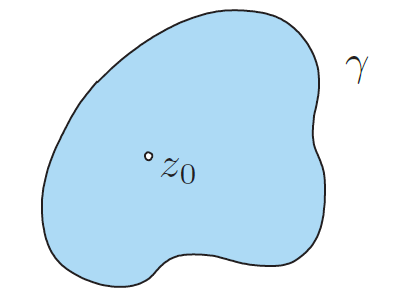
\includegraphics[width=0.3\textwidth]{./SaltChapter/fig-3-0-10}
\end{center}
\end{figure*}

\begin{salt_exercise} \label{ex-3-27}
함수 $F$를 $F(z) = \dfrac{\exp(iz)}{z^2+1}$로 정의하고, $R>1$이라 하자.
\begin{itemize}
\item[(1)]
실수축 위의 점 $-R$부터 $R$까지를 잇는 선분 $S$와
반지름이 $R$이고 $R$에서 $-R$까지를 연결하는 상반평면의 원호 $T$를 연결한 
반원형 닫힌경로를 $\sigma$라고 하자.
다음을 증명하라.
\[
\int_\sigma F(z)dz = \dfrac\pi e.
\]
\item[(2)] $z$가 상반평면의 점일 때, $|\exp(iz)|\le 1$임을 증명하여,
충분히 큰 $|z|$에 대하여 $|F(z)| \le 2/|z|^2$임을 보여라.
\item[(3)] $\lim\limits_{R\to\infty} \dint_T F(z)dz = 0$임을 보여라.
그러면 $\lim\limits_{R\to\infty} \dint_S F(z)dz = \dfrac\pi e$가 된다.
\item[(4)] 결론적으로 $S$를 따른 적분을 매개변수 $x$의 적분으로 표현하면 다음 결과가 얻어짐을 보여라.
\[
\int_{-\infty}^\infty \dfrac{\cos x}{1+x^2}dx := 
\lim_{R\to\infty} \int_{-R}^R \dfrac{\cos x}{1+x^2} dx = \dfrac \pi e.
\]
\end{itemize}
\end{salt_exercise}

\begin{salt_exercise} \label{ex-3-28}
적분 $\dint_0^{2\pi} e^{\cos \theta} \cos(\sin\theta)d\theta$을 구하라.
힌트: 함수 $\exp(\exp(i\theta))$를 생각해보자.
\end{salt_exercise}

\section{복소해석함수는 무한번 미분가능하다}

이 절에서는 영역에 정의된 복소해석함수의 근본적인 성질로서 
무한번 복소미분가능함을 보일 것이다.

이는 실해석의 경우와 대비되는 결과이다.
이미 예제 \ref{example-0-1}에서 살펴본 바와 같이
실함수는 고립점에서 미분가능하지 않을 수 있다.
좀 더 극단적인 현상을 보여주는 예로 
모든 점에서 미분가능하지만, $f'$은 어떤 점에서도 미분이 불가능한 
함수 $f:\mathbb R\to \mathbb R$가 존재한다.
관심있는 독자는 [Gelbaum 과 Olmsted (1964)] %==[salt] 참고문헌
을 찾아보기 바란다.
그 책에서 모든 점에서 연속인 함수 $g:\mathbb R\to \mathbb R$가 
모든 점에서 미분이 불가능한 예를 찾을 수 있는데,
그 적분
\[
f(x) = \int_0^x g(\xi)d\xi, \quad x\in \mathbb R
\]
으로 정의된 $f:\mathbb R\to \mathbb R$는 모든 점에서 미분가능하며,
도함수인 $g$는 어떤 점에서도 미분이 불가능하게 된다.

\begin{salt_corollary} \label{coro-3-6}
\
\begin{itemize}
\item[(1)] $D$가 영역이고,
\item[(2)] $f:D\to\mathbb C$는 $D$에서 복소해석함수이면,
\end{itemize}
$f'$도 $D$에서 복소해석함수이다.
\end{salt_corollary}

이 결과를 이용하면 다음과 같이 연쇄적인 결과를 얻을 수 있음에 주목하자.
\begin{center}
\fbox{$f\in \Hol(D)$} $\Rightarrow$ \fbox{$f'\in \Hol(D)$} $\Rightarrow$
\fbox{$f''\in \Hol(D)$} $\Rightarrow \ \cdots$ 
\end{center}
따라서 $f$가 영역  $D$에서 복소해석함수이면 (즉, $f\in \Hol(D)$),
무한번 복소미분가능하다.

어떻게 증명할지 계획을 만들어보자.
코시 적분공식에서 다음을 알고 있다.
\[
f(z) = \dfrac1{2\pi i} \int_{C_r} \dfrac{f(\zeta)}{\zeta - z} d\zeta,
\]
여기서 $C_r$은 $z$를 중심으로 하고 반지름 $r$인 원이다.
적분기호하에서 형식적인 미분을 적용하면
$f$의 미분에 대한 표현을 얻을 수 있다.
\[
f'(z) = \dfrac1{2\pi i} \int_{C_r} \dfrac{f(\zeta)}{(\zeta - z)^2} d\zeta.
\]
이 식을 증명한 후, 점 $z$와 $w$에서의 미분에 대한 위의 표현을 사용하여, 극한
\[
\lim_{w\to z}\dfrac{f'(w)-f'(z)}{w-z}
\]
이 존재함을 보일 것이다.

{\bf 증명}

$z_0\in D$라 하고,
함수 $g$를 다음과 같이 정의하자.
\[
g(z) = \begin{cases}
\dfrac{f(z)-f(z_0)}{z-z_0}, & z\ne z_0, \\
f'(z_0), & z=z_0.
\end{cases}
\]
$g$가 $D\setminus \{z_0\}$에서 복소해석함수이고, 
$D$에서 연속함수임은 분명하다.
이제 명제 \ref{prop-3-5}에 사용한 기법을 $g$에 적용하자.
원판 $\{z\in\mathbb C\,:\, |z-z_0| \le r\}$이
영역 $D$에 포함되도록 충분히 작은 $r>0$을 고르고
$C_r$을 $z_0$을 중심으로 반지름 $r$인 원을 반시계방향으로 도는 경로라고 하자.
그러면,
\begin{align}
f'(z_0) &= g(z_0)
= \dfrac1{2\pi i} \int_{C_r} \dfrac{g(z)}{z - z_0} dz \nonumber \\
&= \dfrac1{2\pi i} \int_{C_r} \dfrac{f(z)-f(z_0)}{(z-z_0)^2} dz \\
&= \dfrac1{2\pi i} \int_{C_r} \dfrac{f(z)}{(z-z_0)^2} dz
- \dfrac{f(z_0)}{2\pi i} \int_{C_r} \dfrac{1}{(z-z_0)^2} dz \nonumber \\
&= \dfrac1{2\pi i} \int_{C_r} \dfrac{f(z)}{(z-z_0)^2} dz - 0. \label{eq-3-5}
\end{align}
따라서 $C_r$ 내부의 $w$에 대하여 $w\ne z_0$이면, 다음을 얻는다.
\[
f'(w) = \dfrac1{2\pi i}\int_{C_\delta} \dfrac{f(z)}{(z-w)^2}dz
= \dfrac1{2\pi i}\int_{C_r} \dfrac{f(z)}{(z-w)^2}dz,
\]
단, $C_\delta$는  중심 $w$ 반지름 $\delta$인 $C_r$ 내부의 작은 원이다. 
두번째 등식은 코시 적분정리로부터 얻어진다. 왜냐하면,
\[
\dfrac{f(\cdot)}{(\cdot - w)^2}
\]
이 $D\setminus \{w\}$에서 복소해석적이고, 경로 $C_r$과 $C_\delta$가
$D\setminus \{w\}$-호모토픽이기 때문이다.

\begin{figure*}[h!]
\begin{center}
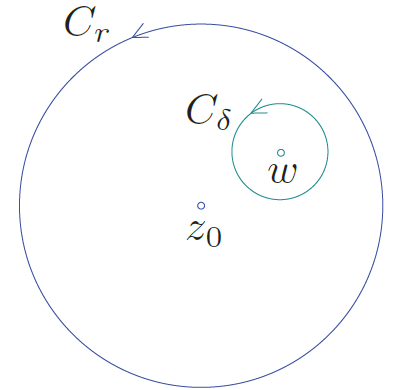
\includegraphics[width=0.3\textwidth]{./SaltChapter/fig-3-0-11}
\end{center}
\end{figure*}

따라서 $C_r$의 내부에서 $w\ne z_0$에 대하여 
\begin{align*}
\dfrac{f'(w)-f'(z_0)}{w-z_0}
&= \dfrac1{w-z_0} \left(
\dfrac1{2\pi i} \int_{C_r} \dfrac{f(z)}{(z-w)^2}dz 
- \dfrac1{2\pi i} \int_{C_r} \dfrac{f(z)}{(z-z_0)^2}dz 
\right) \\
&= \dfrac1{2\pi i}\int_{C_r} \dfrac{f(z)(2z - z_0 -w)}{(z-w)^2(z-z_0)^2} dz.
\end{align*}
만일 $w\approx z_0$이면 이 값은 어떻게 될까?
분자는 
\[
f(z)(2z - z_0 -w) = 2f(z)(z-z_0)
\]
에 분모는 $(z-z_0)^2(z-z_0)^2$에 가깝게 된다.
따라서 다음 결과를 예상해볼 수 있다.
\[
\lim_{w\to z_0} \dfrac{f'(w) - f'(z_0)}{w-z_0} = \dfrac2{2\pi i} \int_{C_r} \dfrac{f(z)}{(z-z_0)^3}dz.
\]
두 값의 차이를 계산해보면,
\[
\lim_{w\to z_0} \dfrac{f'(w) - f'(z_0)}{w-z_0} - \dfrac2{2\pi i} \int_{C_r} \dfrac{f(z)}{(z-z_0)^3}dz
= (w-z_0) \dfrac1{2\pi i} \int_{C_r} \dfrac{(3z-z_0-2w)f(z)}{(z-w)^2(z-z_0)^3}dz.
\]
$z_0$에 가까운 모든 $w$에 대하여 이 적분값이 적당한 상수로 유계이면,
$w-z_0$를 곱한 값은 $w\to z_0$일 때 원하는 만큼 작게 만들 수 있다.
이를 보이기 위해 중심이 $z_0$이고 반지름이 $r$보다 작은, 예를 들면 $r/2$인
원판을  생각하고 $w$를 이 원판 내부로 제한하자 ($w$가 $z_0$의 근방에 있도록).
이제부터 $w$가 다음 콤팩트 집합에 속한다고 할 수 있다.
\[
\left\{ w\in\mathbb C\,:\, |w-z_0| \le \frac r2 \right\}.
\]
연속함수 $\varphi$를
\begin{align*}
(z,w) \stackrel{\varphi}{\mapsto} & \left| \dfrac{(3z-z_0-2w)f(z)}{(z-w)^2(z-z_0)^3} \right| \\
& : C_r \times \left\{w\in\mathbb C\,:\, |w-z_0| \le \frac r2 \right\}
(=: K \subset \mathbb C^2 = \mathbb R^4 ) \to \mathbb R
\end{align*}
라 정의하면 $K$는 $\mathbb R^4$에서 유계인 닫힌집합이므로 콤팩트 집합이다.
따라서 콤팩트 집합 $K$에 정의된 연속함수 $\varphi : K \to \mathbb R$는 
최대값 $M\ge0$을 갖는다.
이제,
\[
\left| \dfrac1{2\pi i}\int_{C_r} \dfrac{f(z)(2z - z_0 -w)}{(z-w)^2(z-z_0)^2} dz \right|
\le \dfrac1{2\pi} M(C_r\text{의 길이}) = \dfrac1{2\pi}M2\pi r = Mr
\]
이므로
\[
\left| \dfrac{f'(w) - f'(z_0)}{w-z_0} - \dfrac2{2\pi i} \int_{C_r} \dfrac{f(z)}{(z-z_0)^3}dz \right|
\le |w-z_0|Mr \stackrel{w\to z_0}{\longrightarrow} 0
\]
가 되어 $f'$이 $z_0$에서 복소미분가능함을 알 수 있다.
$z_0$의 선택을 임의로 할 수 있으므로 $f'$은 영역 $D$에서 복소해석함수이다.
\hfill $\square$

\begin{salt_exercise} \label{ex-3-29}
영역  $D$에서 $f$가 복소해석함수라 하자.
$n\in\mathbb N$에 대하여 $f^{(n)}$이 연속적으로 복소미분가능함이 당연한가?
\end{salt_exercise}

\section{리우비유 정리와 대수학의 기본정리}

복소해석함수와 관련된 엄밀성을 보여주는 예를 하나 더 살펴보자.

\begin{salt_theorem}[리우비유(Liouville) 정리] \label{thm-3-7}
유계인 전해석함수는 상수함수이다.
\end{salt_theorem}

다시 한번 실해석의 경우와 비교해보자.
우리가 잘 아는 함수 $x\to \sin x$의 예를 보면
$\mathbb R$에서 미분가능하며,
모든 $x\in\mathbb R$에 대하여 $|\sin x|\le 1$이므로 
유계이다.
하지만 $\sin$은 상수함수가 아니다.

한편, 리우비유 정리를 적용해보면
전해석함수 $z\mapsto \sin z$는 상수함수가 아니기 때문에
$\mathbb C$에서 유계가 될 수 없다.
앞의 \ref{sec-1-4-2}절에서 확인한 바와 같이,
$y\to\pm\infty$일 때 $|\sin(iy)| \to \infty$이므로,
정의에 따라 직접 계산하는 방법으로도 이를 확인할 수 있다.

{\bf 증명}
모든 $z\in \mathbb C$에 대하여 $|f(z)|\le M$인
상수 $M\ge0$이 존재한다고 하자.
$w\in\mathbb C$이고 $\gamma$가 중심 $w$, 반지름 $R$인 원형 경로하고 하자, 
여기서 $R$은 임의의 양수이다.
그러면 따름정리 \ref{coro-3-6}의 증명에서 (특히, 식 \eqref{eq-3-5}에서)
\[
f'(w) = \dfrac1{2\pi i} \int_\gamma \dfrac{f(z)}{(z-w)^2}dz
\]
이므로
\[
|f'(w)| = \left| \dfrac1{2\pi i} \int_\gamma \dfrac{f(z)}{(z-w)^2}dz \right|
\le \dfrac1{2\pi}\cdot \dfrac M{R^2}\cdot 2\pi R = \dfrac MR
\]
이다.
그런데 $R>0$을 임의로 잡을 수 있으므로 $f'(w)=0$이다.
즉, 모든 $w\in\mathbb C$에 대하여 $f'(w)=0$이 되어 $f$는 상수함수이다.
이미 연습문제 \ref{ex-2-13}에서 증명했지만 다른 방식으로 보이도록 하자.
$z\in\mathbb C$이면, $0$부터 $z$까지 잇는 선분 $\gamma_z$에 대하여
\[
f(z) - f(0) = \int_{\gamma_z} f'(\zeta)d\zeta = 0
\]
가 되어 증명이 끝난다.
\hfill $\square$

이 결과는 대수학의 기본정리에 대한 간단한 증명에 사용될 수 있다.
\footnote{
이름과 달리 완전히 대수적으로만 이 정리를 증명하는 방법은 없다.
증명에는 실수의 완비성이 필요한데 이것은 대수적 개념이 아니기 때문이다.
또한, 현대대수에서 실제로 ``근본적(fundamental)''인 것도 아니다.
이 이름은 붙여진 것은 대수학의 연구가 주로 실계수 또는 복소계수 다항식의 해와 관련되었던
시대이다.}

\begin{salt_corollary} [대수학의 기본정리] \label{coro-3-7}
1차 이상의 모든 다항식은 $\mathbb C$에서 해를 갖는다.
\end{salt_corollary}

$p(z) = x_0 + c_1z + \cdots + c_dz^d$ 
($c_0, c_1, \ldots, c_d\in \mathbb C$, $c_d\ne0$)로 정의된
다항식 $p:\mathbb C \to \mathbb C$에 대하여,
$d$를 $p$의 차수(degree)라 한다. 
$p(z_0)=0$을 만족하는 $z_0\in \mathbb C$를 $p$의 해(zero/root)라 부른다.

{\bf 증명}
$d\ge1$인 다항식 $p(z) = x_0 + c_1z + \cdots + c_dz^d$가
$\mathbb C$에서 해를 갖지 않는다고 하자.
즉, 모든 $z\in\mathbb C$에 대하여 $p(z)\ne0$이다.
그런데 $p$는 전해석함수이고 $0$이 될 수 없으므로 역수를 
함수 $f(z) = 1/p(z)$ ($z\in\mathbb C$)라 정의하면
$f$로 전해석함수이다. 연습문제 \ref{ex-2-6}을 보라.
연습문제 \ref{ex-1-24}에서 다항식의 증가율을 계산했던 결과를 인용하면
\begin{center}
%$|z|>R$이면 $|p(z)|\ge M|z|^d$를 만족하는 $M,R>0$이 존재한다.
$M,R>0$이 존재하여, $|z|>R$이면 $|p(z)|\ge M|z|^d$이다.
\end{center}
콤팩트 집합 $\{z\in\mathbb C\,:\, |z|\le R\}$에서
연속함수 $z\mapsto |p(z)|$는 양의 최솟값 $m$을 갖는다 ($p$가 $0$이 될 수 없으므로).
따라서
\[
|f(z)| \le \max\left\{ \dfrac1{MR^d}, \dfrac1m \right\}, \quad z\in\mathbb C.
\]
리우비유 정리에 의해 $f$는 상수함수가 되어야 한다.
따라서 $p$도 상수가 되어 차수 $d\ge1$이라는 가정에 모순이다.
\hfill $\square$

예를 들면, 다항식 $p(z) = z^{1976} -3z^{28} + \sqrt{399}$의 해가
복소평면 어딘가에 존재함을 보장할 수 있다.

\begin{salt_exercise} \label{ex-3-30}
전해석함수 $f$가 $0$에서 일정한 거리만큼 떨어져 있으면,
(즉, $\delta>0$가 존재하여 모든 $z\in\mathbb C$에 대하여 $|f(z)|\ge\delta$를 만족한다)
$f$가 상수함수임을 보여라.
\end{salt_exercise}

\begin{salt_exercise} \label{ex-3-31}
전해석함수 $f$의 치역이 $\{ w\in\mathbb C\,:\, |w-w_0| < r\}$과 만나지 않으면
$f$는 상수함수임을 보여라.
\end{salt_exercise}

\begin{salt_exercise} \label{ex-3-32}
전해석함수 $f$가 실수축과 허수축 양방향으로 주기성을 가지면 상수함수임을 보여라.
즉, $T_1, T_2\in \mathbb R$이 존재하여 
모든 $z\in \mathbb C$에서 $f(z) = f(z+T_1) =f(z+iT_2)$를 만족한다.
\end{salt_exercise}

\begin{salt_exercise} \label{ex-3-33}
전해석함수의 이론에서 다루는 고전적 주제는
$|z|$가 커짐에 따라 $|f|$가 어떻게 증가하는지에 따라 전해석함수 $f$를 규정하는 것이다.
예를 한가지 보자.
\begin{itemize}
\item[(1)] 전해석함수 $f$가 모든 $z\in\mathbb C$에 대하여 
$|f(z)| \le |\exp z|$를 만족하면, 
$|c|\le1$인 상수 $c$가 존재하여 $f$는 $c\cdot \exp z$가 됨을 보여라.
(따라서 상수함수가 아닌 전해석함수가 지수함수보다 빠르지 않게 증가한다면
실제로 지수함수가 된다)
\item[(2)] ``다항식은 지수함수보다 천천히 증가하지만 $p\ne \exp z$''라는 근거로
위의 결과가 옳지않다는 성급한 주장을 할 수 있다.
모든 $z\in\mathbb C$에 대하여 $p$가 $|p(z)|\le |\exp z|$를 만족한다면
$p\equiv0$임을 보여 이 주장에서 논리적으로 틀린 부분을 찾아라. \\
힌트: $z=x<0$인 경우를 생각하자.
\end{itemize}
\end{salt_exercise}

\begin{salt_exercise} \label{ex-3-34}
$f:\mathbb C \to \mathbb C$가 전해석함수라고 하자.
중심이 $0$이고 반지름 $R>0$인 원을 반시계방향으로 한바퀴 도는 원형경로 $C$의
내부에 복소수 $a_1, a_2$가 있으며 $a_1\ne a_2$라 가정하자.
\begin{itemize}
\item[(1)] $\left| \dint_C \dfrac{f(z)}{(z-a_1)(z-a_2)}dz \right| \le
\dfrac{2\pi R}{(R-|a_1|)(R-|a_2|)} \max\limits_{z\in C} |f(z)|$를 증명하라.
\item[(2)] 모든 $z\in \mathbb C$에 대하여
$\dfrac1{(z-a_1)(z-a_2)} = \dfrac\alpha{z-a_1} + \dfrac\beta{z-a_2}$를 만족하는
$\alpha, \beta \in \mathbb C$를 구하라.
\item[(3)] 적분 $\dint_C \dfrac{f(z)}{(z-a_1)(z-a_2)}dz$을
$\dint_C \dfrac{f(z)}{z-a_1}dz$와 $\dint_C \dfrac{f(z)}{z-a_2}dz$로 나타내고,
코시 적분공식을 이용하여 식을 간단히 정리하라.
\item[(4)] 위 결과를 이용하여 리우비유 정리를 증명하라.
\end{itemize}
\end{salt_exercise}

\section{모레라 정리: 코시 적분정리의 역}

 코시 적분정리를 다시 돌아보자.
\begin{itemize}
\item[(1)] $D$가 영역이고, 
\item[(2)] $f:D\to \mathbb C$는 \textcolor{red}{복소해석함수}이고,
\item[(3)] $\Delta$는 $\Delta \subset D$의 임의의 원판이고,
\item[(4)] $\gamma$는 $\Delta$ 내부의 조각적으로 매끄러운 닫힌 경로이면,
\end{itemize}
\[
\int_\gamma f(z)dz = 0.
\]
이제 다음과 같이 그 역도 성립함을 보일 것이다.
\begin{salt_theorem}[모레라 정리] \label{thm-3-8}
\
\begin{itemize}
\item[(1)] $D$가 영역이고, 
\item[(2)] $f:D\to \mathbb C$는 \textcolor{red}{연속함수}이고,
\item[(3)] $D$에 속하는 모든 닫힌 사각형 경로 $\gamma$에 대하여
\[
\int_\gamma f(z)dz = 0
\]
이면,
\end{itemize}
$f$는 $D$에서 \textcolor{red}{복소해석함수}이다.
\end{salt_theorem}
다시 말하면, 특별한 경로적분들이 $0$이면
$f$가 복소해석함수라는 결론을 얻는다!

{\bf 증명}

$z_0\in D$, $\Delta$는 중심이 $z_0$이고 $\Delta \subset D$인 원판이고,
$\gamma_{z_0,z}$는 $z_0$에서 수평방향으로 먼저 진행한 후
수직방향으로 움직여 $z$에 도달하는 경로라고 하자.
\begin{figure*}[h!]
\begin{center}
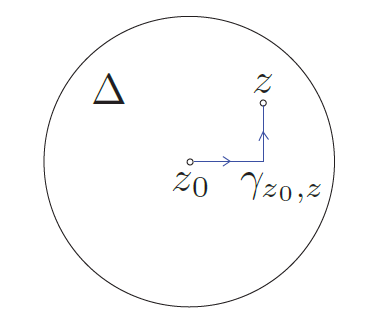
\includegraphics[width=0.3\textwidth]{./SaltChapter/fig-3-0-12}
\end{center}
\end{figure*}

$F:\Delta \to \mathbb C$를 $F(z) = \dint_{\gamma_{z_0,z}} f(\zeta)d\zeta$, $z\in\Delta$로
정의하자.

이제 $F$가 $\Delta$에서 복소해석함수이고, 그 미분이 $f$가 됨을 보일 것이다.
이로써 $f$가 $\Delta$에서 복소해석함수임이 증명된다. 왜?
$f$가 복소해석함수의 도함수이므로 따름정리 \ref{coro-3-6}에 의해
$D$에서 복소해석함수이다.

$z\in \Delta$가 주어졌고, $\epsilon>0$이라 가정하자.
$f$가 연속이므로, $\delta>0$가 존재하여
$|w-z|<\delta$와 $w\in \Delta$를 만족할 때마다
$|f(w) - f(z)| <\epsilon$가 성립한다.
\[
F(w) - F(z) = \int_{\gamma_{z_0,w}} f(\zeta) d\zeta
- \int_{\gamma_{z_0,z}} f(\zeta) d\zeta
\]
이므로
닫힌 사각형 경로에서 $f$의 적분이 $0$임을 이용하면 다음을 얻는다.
\[
F(w) - F(z) = \int_{\gamma_{z,w}} f(\zeta) d\zeta,
\]
여기서 $\gamma_{z,w}$는 $z$에서 수평방향으로 먼저 진행한 후
수직방향으로 움직여 $w$에 도달하는 경로이다.
예를 들어 아래 그림의 적분 경로에서는 다음과 같이 계산된다 (피적분함수는 생략하고 쓰면).
\begin{align*}
F(w) - F(z) 
&= \int_{\gamma_{z_0,w}} f(\zeta) d\zeta
- \int_{\gamma_{z_0,z}} f(\zeta) d\zeta
= \cancel{\int_A} + \int_B + \int_C - \left(\cancel{\int_A} + \int_D \right) \\
&= \underbrace{\int_B + \int_C + \int_{-\gamma_{z,w}} + \int_{-D}}_{=0}
+\int_{\gamma_{z,w}} f(\zeta) d\zeta.
\end{align*}

\begin{figure*}[h!]
\begin{center}
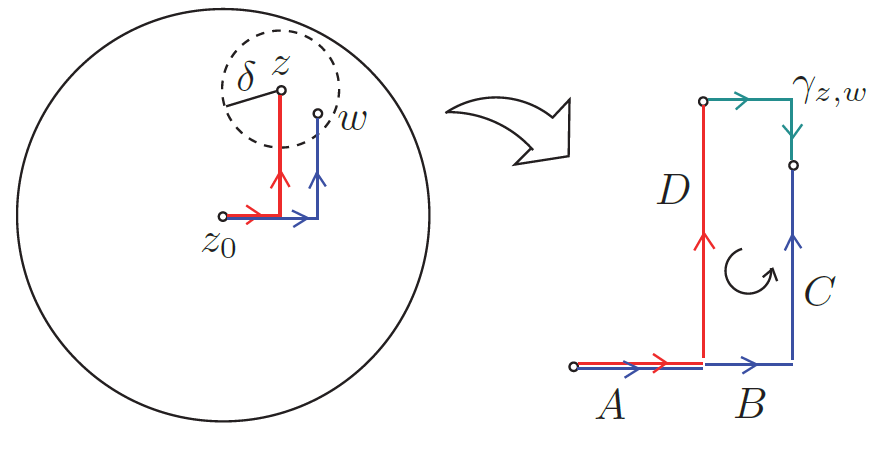
\includegraphics[width=0.5\textwidth]{./SaltChapter/fig-3-0-13}
\end{center}
\end{figure*}

따라서 $0<|w-z|<\delta$에 대하여, 다음을 얻는다.
\begin{align*}
\frac{F(w)-F(z)}{w-z} - f(z)
&= \dfrac1{w-z}\int_{\gamma_{z,w}} f(\zeta)d\zeta - f(z) \dfrac1{w-z}\int_{\gamma_{z,w}} 1 d\zeta \\ 
& = \int_{\gamma_{z,w}} (f(\zeta) - f(z)) d\zeta.
\end{align*}
여기서 
\[
\int_{\gamma_{z,w}} 1 d\zeta = w-z
\]
를 얻기위해 복소해석함수 $1$에 대하여 경로적분의 기본정리를 사용하였다.
결론적으로 위의 결과와 경로 $\gamma_{z,w}$의 길이가
\[
|\Re(w-z)| + |\Im(w-z)| \le 2|w-z|
\]
를 만족한다는 성질로부터 다음을 얻는다.
\begin{align*}
\left| \frac{F(w)-F(z)}{w-z} - f(z) \right|
&= \left| \dfrac1{w-z} \int_{\gamma_{z,w}} (f(\zeta) - f(z)) d\zeta \right|  \\
&< \dfrac\epsilon{|w-z|} (|\Re(w-z)| + |\Im(w-z)|) \le 2\epsilon.
\end{align*}
이로써 증명이 끝난다.
\hfill $\square$

\section{참고}

정리 \ref{thm-3-4}의 증명은 [Beck, Marchesi, Pixton, Sabalka (2008)]의 설명을
거의 따랐다. 연습문제 \ref{ex-3-3}, \ref{ex-3-4}, \ref{ex-3-12}, \ref{ex-3-20}, \ref{ex-3-27}은
[Beck, Marchesi, Pixton, Sabalka (2008)]에서 가져왔다.
연습문제 \ref{ex-3-10}, \ref{ex-3-14}, \ref{ex-3-18}, \ref{ex-3-19}, \ref{ex-3-22}, \ref{ex-3-24}는
[Needham (1997)]을 인용하였다.
연습문제 \ref{ex-3-21}은 [Rudin (1987)]에서, 
연습문제 \ref{ex-3-26}, \ref{ex-3-33}, \ref{ex-3-34}는 [Flanigan (1972)]에서,
연습문제 \ref{ex-3-28}은 [Howie (2003)]에서 각각 가져왔다.

